\chapter{Diffusion and Depletion Methods} \label{Sec:diffusion}

The previous chapter developed methods for solving the transport equation for a couple important scenarios. The first is on the length scale of a unit cell for a fine-group structure using the collision probability and response matrix methods. The second is for the length scale of an assembly where the discrete ordinates method is presented.

This chapter discusses how to stitch together the assembly calculations to compute the neutron flux distribution across the entire reactor core. Until recently, using transport-based methods on the full core was prohibitive except for benchmarking calculations. Even with modern resources, such calculations are still quite expensive. Therefore, we often employ neutron diffusion-based approaches using a few energy groups.






%%%%%%%%%%%%%%%%%%%%%%%%%%%%%%%%%%%%%%%%%%%%%%%%%%%%%%%%%%%%%%%%%%%%%%%%%%%%%%%%
\section{Leakage Spectrum and Buckling}

The first consideration we must handle is that the assembly calculation employ reflecting boundary conditions, implying the calculation treats the assembly in an infinitely repeated array. In an actual reactor, the materials within assemblies varies throughout the reactor core. For example, after several refueling cycles, a reactor contains assemblies with fresh fuel and fuel that have been through the one or more cycles. The fuel assemblies that have undergone the most burnup are typically unable to sustain a chain reaction, even if we were to stack an infinite number of them into a lattice. Therefore, the reactivity needed to achieve criticality comes from fresh and less-burned fuel assemblies that are interspersed into some arrangement. 

Stated another way, the most reactive fuel assemblies would be supercritical placed in an infinite array and the least reactive ones would be subcritical. The overall criticality of the system is established by neutrons from more reactive assemblies feeding less reactive ones in a way such that the overall neutron population is balanced. This flow of neutrons impacts the flux spectra within the different assembly types, which in turn impacts the few group cross sections and diffusion coefficients.




\subsection{Buckling}

Since the effect on the spectrum is from by leakage, we are motivated to find a way to mathematically balance the neutron population within each assembly in a way that accounts for leakage. The way this is done is through the theory of \emph{buckling}, where $B^2$ is a parameter (eigenvalue) that achieves this. One may recall from buckled neutron diffusion theory that
\begin{align}
  B^2 D = \text{ effective leakage ``cross section'' for a diffusive system,} \nonumber
\end{align}
where $B^2$ is the (geometric) buckling having units of per area---the diffusion coefficient $D$ has units of length. To apply the mathematical machinery of buckling however, we require that the system have uniform material properties or be homogenized and be sufficiently large so that we can apply the zero flux boundary condition. (There are extrapolation distances that account for the actual boundary conditions, but these are limited to the one-speed approximation.)

In a critical, finite-sized system, $B^2 > 0$. Then $B^2 D$ can be interpreted a removal term that accounts for neutrons leaking out of the system in an average sense within a homogenized infinite media. Stated another way, if the critical system is modeled as infinite and is supercritical in this configuration, we need to apply a positive $B^2 D$ leakage term to remove the neutrons to match criticality. 

We can also consider the case where a system is infinite and subcritical. To achieve neutron balance we would need to add neutrons from the outside via a source. This can be modeled by adding a $B^2 D$ term onto the source (right-hand) side of the neutron balance equation. We could then move this to the left-hand side and have a negative loss term.

So with respect to an infinite, homogenized assembly, the buckling satisfies:
\begin{itemize}
  \item $B^2 > 0$, \quad net outflow (leakage) needed to achieve neutron balance,
  \item $B^2 = 0$, \quad neutron balance is achieved naturally, 
  \item $B^2 < 0$, \quad net inflow needed to achieve neutron balance.
\end{itemize}
The similarity to the effective multiplication factor $k$ should be apparent with the mapping of these cases to supercritical $(k > 1)$, critical $(k = 1)$, and subcritical $(k < 1)$ homogenized mixtures. In fact, like the effective multiplication factor, $B^2$ is the fundamental eigenvalue that for a given value $k$. The task at hand is to find the value of $B^2$ that makes $k = 1$. The energy-dependence of the eigenfunction to this problem then can be used to obtain the effect of leakage on the energy spectrum.

Note that $B^2$ can be either be positive or negative. This implies that $B$ is either real or imaginary. The real case corresponds to a critical or supercritical homogenized assembly and the imaginary case to the subcritical case. This can be thought of in the context of the complex exponential $e^{iBx}$, where real values imply the spatial function is given by trigonometric functions $\cos(Bx)$ and imaginary values correspond to exponential or hyperbolic trigonometric functions $\cosh(\kappa x)$.




\subsection{Continuous-Energy B$_N$ Equations}

The mathematical problem we solve to find the fundamental eigenvalue $B^2$ is generally given by the B$_N$ equations. Typically for light-water reactor analysis, a low-order version B$_1$ is used.

We begin with the 1-D planar transport equation with spatially constant cross sections assumed:
\begin{align}
  \left[ \mu \frac{d}{dx} + \Sigma_t \right] \psi(x,\mu,E) = \sum_{\ell=0}^\infty \left( \frac{2\ell + 1}{2} \right) P_\ell(\mu) \int_0^\infty \Sigma_{s\ell}(E' \rightarrow E) \psi_\ell(x,E') dE' + s(x,E) .
\end{align}
Here we expanded the scattering source into Legendre moments and defined $s(E)$ as the fission source. (In the previous chapters we use $Q$, but alas, there is a different function that uses this symbol in this section.)

Because the cross sections are spatially constant and if we can approximate the flux moments as zero at the boundaries of the slab (reasonable for geometrically large systems), we can show that the angular flux and fission source satisfy the following functional form:
\begin{subequations}
\begin{align}
  \psi(x,\mu,E) &= \Psi(\mu,E) e^{i B x}, \\
  s(x,E) &= S(E) e^{i B x}.
\end{align}
\end{subequations}
Here we refer to $\Psi$ and $S$ as the angular flux and source spectra. 

Inserting these into the transport equation, solving for the collision rate, and expanding out the fission source we get
\begin{align}
  \Sigma_t(E) \Psi(\mu,E) 
  &= \sum_{\ell=0}^\infty \left( \frac{2\ell + 1}{2} \right) \frac{ P_\ell(\mu) }{ 1 + i B \mu / \Sigma_t(E) } \int_0^\infty \Sigma_{s\ell}(E' \rightarrow E) \Psi_\ell(E') dE' \nonumber \\
  &+ \frac{1}{k} \frac{  \chi(E) }{ 2 ( 1 + i B \mu / \Sigma_t(E) ) } \int_0^\infty \nu\Sigma_f(E') \Psi_0(E') dE' .
\end{align}
Here we define the $\ell$th Legendre moment of the angular flux spectrum in the traditional manner:
\begin{align}
  \Psi_\ell(E) = \int_{-1}^1 P_\ell(\mu) \Psi(\mu,E) d\mu .
\end{align}

Taking inspiration from the $P_N$ equations, we multiply this equation by $P_n(\mu)$ to obtain an infinite number of equations for the Legendre moments of the angular flux spectra:
\begin{align}
  \Sigma_t(E) \Psi_n(E) 
  &= \sum_{\ell=0}^\infty ( 2 \ell + 1 ) A_{n\ell}(E) \int_0^\infty \Sigma_{s\ell}(E' \rightarrow E) \Psi_\ell(E') dE' \nonumber \\
  &+ \frac{1}{k} \delta_{n0} A_{n0}(E) \chi(E) \int_0^\infty \nu\Sigma_f(E') \Psi_0(E') dE' , \quad n \ge 0. \label{Eq:diffusion_BNEquations_infinite}
\end{align}
Here we define the coefficient:
\begin{align}
  A_{n\ell}(E) = \frac{1}{2} \int_{-1}^1 \frac{ P_n(\mu) P_\ell(\mu) }{ 1 + i B \mu / \Sigma_t(E) } d\mu .
\end{align}

This coefficient $A_{n\ell}$ satisfies a few important properties. First, we can define the zeroth-order coefficients,
\begin{subequations}
\begin{align}
  A_{00} &= -\frac{\Sigma_t}{i B} \tanh^{-1} \left( -\frac{\Sigma_t}{i B} \right) = -\frac{\Sigma_t}{i B} Q_0 \left( -\frac{\Sigma_t}{i B} \right) , \\
  A_{0n} &= -\frac{\Sigma_t}{i B} Q_n \left( -\frac{\Sigma_t}{i B} \right) ,
\end{align}

in terms of a special function $Q_n$, which is the \emph{Legendre function of the second kind} (we discuss this shortly). We can clearly see that the coefficient is symmetric,
\begin{align}
  A_{n\ell} = A_{\ell n} .
\end{align}
Also, we can show that they satisfy the following recurrence relation:
\begin{align}
  (2\ell + 1) \frac{\Sigma_t}{iB} A_{n \ell} + ( \ell + 1 ) A_{n,\ell+1} + \ell A_{n,\ell-1} = \frac{\Sigma_t}{iB} \delta_{n\ell}.
\end{align}
\end{subequations}
Using this relationship, for a given $A_{n0}$, we can determine the other coefficients $A_{n\ell}$ for $\ell = 1, \ldots, n$.

As promised we now discuss the Legendre function of the second kind $Q_n$. We are already (mostly) familiar with the Legendre function of the first kind $P_n$, which for integer $n$ are simply the Legendre polynomials. The Legendre function of the second kind for complex argument $z$ is defined by the following integral:
\begin{align}
  Q_n(z) = \frac{1}{2} \int_{-1}^1 \frac{ P_n(t) }{ z - t } dt .
\end{align}
They follow the recurrence relations:
\begin{subequations}
\begin{align}
  &( 2n + 1 ) z Q_n(z) = ( n + 1 ) Q_{n+1}(z) + n Q_{n-1}(z), \\
  &P_n(z) Q_{n-1}(z) - P_{n-1}(z) Q_n(z) = \frac{1}{n} , \quad n \ge 1.
\end{align}
\end{subequations}

To obtain the $B_N$ equations, we truncate the scattering order at $n = N$ in Eq.~\eqref{Eq:diffusion_BNEquations_infinite}. We then multiply by $(2n + 1)z$ and apply the recurrence relationships. After much algebra, we arrive at the following (infinite) system of equations:
\begin{subequations}
\begin{align}
  \frac{i}{B} ( 2n + 1 ) \Sigma_t(E) \Psi_{n}(E) 
  &= (n+1) \Psi_{n+1}(E) + n \Psi_{n-1}(E) \nonumber \\*
  &+ \frac{i}{B} ( 2n + 1 ) \int_0^\infty \Sigma_{sn}(E' \rightarrow E) \Psi_n(E') dE' \nonumber \\*
  &+ \frac{1}{k} \frac{i}{B} \delta_{n0} \chi(E) \int_0^\infty \nu\Sigma_f(E') \Psi_n(E') , \quad 0 \le n \le N, \\
\frac{i}{B} ( 2n + 1 ) \Sigma_t(E) \Psi_{n}(E) &= (n+1) \Psi_{n+1}(E) + n \Psi_{n-1}(E)  , \quad n > N .
\end{align}
\end{subequations}
Each of the Legendre moments $\Psi_n$ measures the amount of anisotropy of the angular flux spectrum. We note that for orders $n \le N$, the source of anisotropy is driven by streaming between different orders and the anisotropic scattering within the same order. For $n > N$, the anisotropy in the angular flux is driven simply by streaming of neutrons.

We often truncate this infinite system of equations at order $N$ to form the B$_N$ equations. Using the definition of the coefficients $A_{n\ell}$ we can arrive at a closure in terms of the Legendre functions of the second kind,
\begin{align}
  \Psi_{N+1} = \frac{ Q_{N+1}( -\Sigma_t / (iB) ) }{ Q_{N}( -\Sigma_t / (iB) ) } \Psi_N
\end{align}
Applying this closure, we can write the B$_N$ equations as
\begin{align}
  &\frac{ n + 1 }{ 2n + 1 } i B \Psi_{n+1}(E) + \frac{ n }{ 2n + 1 }  i B \Psi_{n-1}(E) + \Sigma_t \Psi_n(E) \nonumber \\*
  &= \int_0^\infty \Sigma_{sn}(E' \rightarrow E) \Psi_n(E') dE' \nonumber \\*
  &+ \frac{1}{k} \delta_{n0} \chi(E) \int_0^\infty \nu\Sigma_f(E') \Psi_n(E') , \quad n = 0, \ldots, N-1, \nonumber \\
  &\frac{ N }{ 2N + 1 }  i B \Psi_{n-1}(E) + \gamma_N(E) \Sigma_t \Psi_n(E) = \int_0^\infty \Sigma_{sN}(E' \rightarrow E) \Psi_N(E') dE' ,
\end{align}
where
\begin{align}
  \gamma_N(E) = 1 + \frac{ N + 1 }{ 2N + 1 } \frac{iB}{\Sigma_t} \frac{ Q_{N+1}(-\Sigma_t/(iB)) }{ Q_{N}(-\Sigma_t/(iB)) } .
\end{align}

If we inspect these equations, we note that they look very similar to the P$_N$ equations in slab geometry except for the following differences:
\begin{align}
   &i B \rightarrow \frac{d}{dx} , \nonumber \\
   &\gamma_N \rightarrow 1. \nonumber
\end{align}
The first of these arises from applying the buckling approximation, which is valid for an homogeneous medium with the approximation of zero-flux moment boundaries. The presence of the additional $\gamma_N$ factor arises because of the closure that handled higher-order anisotropy beyond the truncation of the scattering order. We can think of the product of $\gamma \Sigma_t$ as a type of transport-corrected cross section, and indeed these two ideas are somewhat related.

As mentioned, the most important case of the B$_N$ equations is where $N = 1$. We note that the zeroth and the first moments are the respective flux and current spectra. However, we can show that $\Psi_0(E)$ is real and $\Psi_1(E)$ is pure imaginary. To ensure the physical quantities we are seeking are real, we define
\begin{subequations}
\begin{align}
  \phi(E) &= \Psi_0(E), \\
  J(E) &= i \Psi_1(E).
\end{align}
\end{subequations}
We then have the following system of two equations:
\begin{subequations}
\begin{align}
  & B J(E) + \Sigma_t(E) \phi(E) = \int_0^\infty \Sigma_{s0}(E' \rightarrow E) \phi(E') dE' \nonumber \\*
  &+ \frac{1}{k} \chi(E) \int_0^\infty \nu\Sigma_f(E') \phi(E'), \\
  & \gamma(E) \Sigma_t(E) J(E) - \int_0^\infty \Sigma_{s1}(E' \rightarrow E) J(E') dE' = \frac{B}{3} \phi(E) .
\end{align}
\end{subequations}
Here we denote $\gamma_1 = \gamma$, which is conventional. We can explicitly evaluate the Legendre function of the second kind in terms of real functions to determine $\gamma$ as
\begin{align}
  \gamma(E) = \left\{ \begin{array}{l l}
  \dfrac{ \dfrac{B}{\Sigma_t}  \tan^{-1} \left( \dfrac{B}{\Sigma_t} \right) }{ 3 \left[ 1 - \dfrac{\Sigma_t}{B} \tan^{-1} \left( \dfrac{B}{\Sigma_t} \right) \right] }, & \quad B^2 \ge 0 , \vspace{0.4em} \\
  \dfrac{ \dfrac{|B|}{\Sigma_t} \ln \left| \dfrac{ 1 + |B|/\Sigma_t }{ 1 - |B|/\Sigma_t } \right| }{ 3 \left[ \dfrac{\Sigma_t}{|B|} \ln \left| \dfrac{ 1 + |B|/\Sigma_t }{ 1 - |B|/\Sigma_t } \right| - 2 \right] }, & \quad B^2 < 0 . \\ \end{array} \right.  
\end{align}
The limiting case of $B^2 = 0$, an infinite medium, is $\gamma = 1$, in which case there is no anisotropy resulting from streaming.




\subsection{Solution of the Multigroup B$_1$ Equations}

The B$_1$ equations can be expressed in multigroup form as follows:
\begin{subequations}
\begin{align}
  &B J_g +  \Sigma_{tg} \phi_g - \sum_{g'=1}^G \Sigma_{s0,g' \rightarrow g} \phi_{g'} 
  = \frac{1}{k} s_g, \\
  &\left[ \gamma_g \Sigma_{tg} - \Sigma_{s1,g \rightarrow g} \right] J_g  - \sum_{\substack{g' = 1\\ g' \ne g}}^G \Sigma_{s1,g' \rightarrow g} \phi_{g'} = \frac{B}{3} \phi_g .
\end{align}
\end{subequations}
Here we normalize the fission source to be one.

We can write the these equations in matrix vector form as
\begin{subequations}
\begin{align}
  B \mathbf{j} + \boldsymbol\Sigma_R \boldsymbol\phi &= \frac{1}{k} \mathbf{s} , \\
  \boldsymbol\Sigma_{tr} \mathbf{j} &= \frac{B}{3} \boldsymbol\phi . \label{Eq:diffusion_B1Current_MatrixVector}
\end{align}
\end{subequations}
Here $\boldsymbol\Sigma_{R}$ and  $\boldsymbol\Sigma_{tr}$ are a \emph{full} matrices given by
\begin{subequations}
\begin{align}
  \boldsymbol\Sigma_{R} &= \left[ \begin{array}{c c c}
  \Sigma_{t1} - \Sigma_{s0, 1 \rightarrow 1} & -\Sigma_{s0,2 \rightarrow 1} & \cdots \\
  -\Sigma_{s0,1 \rightarrow 2} & \Sigma_{t2} - \Sigma_{s0, 2 \rightarrow 2} & \cdots \\
  \vdots & \vdots & \ddots \\ \end{array} \right] , \\
  \boldsymbol\Sigma_{tr} &= \left[ \begin{array}{c c c}
  \gamma_1(B) \Sigma_{t1} - \Sigma_{s1, 1 \rightarrow 1} & -\Sigma_{s1,2 \rightarrow 1} & \cdots \\
  -\Sigma_{s1,1 \rightarrow 2} & \gamma_2(B) \Sigma_{t2} - \Sigma_{s1, 2 \rightarrow 2} & \cdots \\
  \vdots & \vdots & \ddots \\ \end{array} \right] ,
\end{align}
\end{subequations}
$\mathbf{j}$ and $\boldsymbol\phi$ are a column vector of group currents and scalar fluxes respectively, and $\mathbf{s}$ is the fission source (column) vector. Here we specifically note that the group $\gamma_g$ explicitly depends on the buckling $B$. Inspired by Fick's law we can define the matrix of diffusion coefficients by taking the inverse of the transport cross section matrix:
\begin{align}
  \mathbf{D} = \frac{1}{3} \boldsymbol\Sigma_{tr}^{-1} .
\end{align}
We can solve for the currents,
\begin{align}
  \mathbf{j} = \frac{B}{3} \boldsymbol\Sigma_{tr}^{-1} \boldsymbol\phi = B \mathbf{D} \boldsymbol\phi ,
\end{align}
and then obtain a linear system for the fluxes:
\begin{align}
  \left[ B^2 \mathbf{D} + \boldsymbol\Sigma_R \right] \boldsymbol\phi = \frac{1}{k} \mathbf{F} \boldsymbol\phi, \label{Eq:diffusion_B1Diffusion_MatrixVector}
\end{align}
where here we write the fission source $\mathbf{s}$ in terms of the fluxes with $\mathbf{F}$ being a full matrix for the emission of fission neutrons.

If we inspect this linear system in Eq.~\eqref{Eq:diffusion_B1Diffusion_MatrixVector} closely, we see that we have a problem. The unknown buckling $B^2$ is within the diffusion matrix $\mathbf{D}$ by way of the $\gamma_g$. This means we have a nonlinear dependence on the buckling to obtain the eigenvalue $k$. This means we need to solve the problem iteratively using a technique such as Newton-Raphson.

As mentioned earlier, the goal here is to find $B^2$ such that $k = 1$ or equivalently $y = k - 1 = 0$. If we guess a value of $B^2$, we can then solve for the fundamental eigenvalue $k$ using a technique such as the power iteration method. We typically first guess $B^2 = 0$ and determine whether $k > 1$ or $k < 1$. This tells us whether we require $B^2 > 0$ or $B^2 < 0$, respectively. We then take a second guess of $B^2$ and solve for a new value of $k$. We call the two values $k_1$ and $k_2$ for the guesses, which allows us to compute the slope. Given the slope we can estimate the value of $B^2$ such that $k = 1$. We try this new guess, and keep doing this until we converge $B^2$ to within some tolerance.

Once we have the flux spectrum $\boldsymbol\phi$ and buckling $B^2$, we can find the current spectrum $\mathbf{j}$ solving the linear system Eq.~\eqref{Eq:diffusion_B1Current_MatrixVector} using Gaussian elimination. 




\subsection{Spectral Expansion and Assembly Homogenization}

The B$_1$ method determines the leakage-corrected flux and current spectra. These require assembly-homogenized cross sections on a fine energy grid, or at least one finer than what would typically be used for a transport calculation on an assembly. This section answers the question of how to use the transport calculations covered in the previous chapter to find these homogenized cross sections.

To review, we first perform slowing down calculations using highly resolved cross sections along with rational approximations and Dancoff factors to obtain self-shielded, fine-group cross sections for each material type. 

These fine-group cross sections are then used as input for detailed transport calculations on reactor unit cells, typically done using the collision probability method. The collision probability calculations provide a detailed flux spectrum with a fine energy resolution, but for the case of a single unit cell surrounded by a large number of typical unit cells (approximated by the buffer zone). We then homogenize each unit cell type and use the transmission probability method with the response matrices to determine the effect of coupling between the unit cells that estimates the impact on the fine energy spectra.

While the response matrix coupling is adequate to adjust the energy dependence of the detailed flux spectra within the unit cell, it is not particularly good at determining the flux shape across the assembly. Capturing this detailed spatial dependence can only really be done through a transport calculation, which would normally be computationally expensive using a fine energy group. To address this computational expense, we condense the the fine group response matrix spectra into coarse group cross sections within each region in the assembly. We then perform a detailed transport calculation across the assembly using these coarse group cross sections---typically this is done using the method of characteristics or the discrete ordinates method. The result of the assembly transport calculation is a spatially detailed flux distribution with coarse energy groups. 

Typically the coarse group structure is not fine enough for the B$_1$ method, so we must perform a flux spectrum expansion. This combines the spatially detailed, coarse-group flux spectra with the fine-group spectra. Let $\phi_{A,i,h}$ be the scalar flux from the assembly calculation within the $i$th spatial cell for coarse group $h$ and let $\phi_{R,I,g}$ be the flux spectrum from the response matrix calculation in the coarse region $I$ where $i \in I$ and on fine group $g$. We can get the expanded flux spectra on the fine groups using
\begin{align}
  \phi_{i,g} = \phi_{A,i,h} \dfrac{ \phi_{R,I,g} }{ \displaystyle\sum_{g \in h} \phi_{R,I,g} } .
\end{align}
The ratio is the relative scalings of of the fine group spectra within the coarse group. We then find the flux weighted homogenized cross sections using
\begin{align}
  \Sigma_{x,g} = \dfrac{ \displaystyle\sum_i \Sigma_{x,i,g} \phi_{i,g} V_i }{ \displaystyle\sum_i \phi_{i,g} V_i },
\end{align}
where $\Sigma_{x,i,g}$ is the fine-group cross section of reaction $x$ in spatial cell $i$ and $V_i$ is the volume of that cell.

Note that there is no requirement for the B$_1$ calculation to use the same group structure as the fine-group calculation. We could perform another condensation to get to a different group structure if we desire.


\subsection{Few-Group Coefficients}

The B$_1$ calculation provides a fine-group flux spectrum $\phi_{B,g}$  and current spectrum $J_{B,g}$ on the homogenized assembly. This is then used to compute cross sections and diffusion coefficients on a few group (often  two, fast and thermal). Here we let $c$ be the group index of this few-group structure. The reaction cross sections are flux-weighted,
\begin{align}
  \Sigma_{x,c} = \dfrac{ \displaystyle\sum_{ g \in c } \Sigma_{x,g} \phi_{B,g} }{ \displaystyle\sum_{ g \in c } \phi_{B,g} } .
\end{align}

The transport cross sections and diffusion coefficients, however, should be weighted by the current spectrum to be consistent with the B$_1$ equations. We first define the current-weighted total cross section as
\begin{align}
  \Sigma_{t1,c} = \dfrac{ \displaystyle\sum_{ g \in c } \gamma_g \Sigma_{t,g} J_{B,g} }{ \displaystyle\sum_{ g \in c } J_{B,g} } .
\end{align}
The few group-to-group P$_1$ scattering cross section is
\begin{align}
  \Sigma_{s1,c' \rightarrow c} = \dfrac{ \displaystyle\sum_{ g' \in c' } \displaystyle\sum_{ g \in c } \Sigma_{s1,g' \rightarrow g} J_{B,g'} }{ \displaystyle\sum_{ g' \in c' } J_{B,g'} } .
\end{align}
We use the current-weighted total cross section and within-group cross section to find the few-group transport cross section:
\begin{align}
  \Sigma_{tr,c} = \Sigma_{t1,c} - \Sigma_{s1,c \rightarrow c} .
\end{align}
The diffusion coefficient is then
\begin{align}
  D_c = \frac{1}{3 \Sigma_{tr,c} } .
\end{align}




\section{Assembly Discontinuity Factors}

In the previous section we discuss how to compute assembly-homogenized cross sections and diffusion coefficients from the detailed heterogeneous assembly flux calculation. This homogenization process introduces significant errors for which the reasons are not entirely obvious and the remedy is counterintuitive. 

In short, the homogenization does not preserve the net currents between assemblies. To preserve both the reaction rates and the net currents, both in an integral sense, we do something that seems a bit crazy: in the diffusion calculation we relax the requirement that the scalar fluxes across assembly interfaces be continuous by using of an \emph{assembly discontinuity factor} that gives improved partial currents. 

Before getting into the reasons why, we note a key point that the discontinuity factor does not account for the influence of heterogeneities within the assembly impacting neighboring assemblies. This is mostly a second-order effect, whereas getting the bulk surface currents right is of first order.

Another nomenclature point is that the idea matching currents is called equivalence theory, borrowing the identical naming for drawing relationships between heterogeneous unit cells and infinite homogeneous media for computing self-shielded cross sections. The idea is very similar here, except at the assembly scale and the goal now is to preserve reaction rates and currents.



\subsection{Rationale}

Why discontinuity factors are used is not obvious at all. In fact, it was not until the 1980s that such ideas become practice in reactor analysis methods.

To understand the motivation, we return to the fact that we have a transport calculation (using method of characteristics or discrete ordinates) on the heterogeneous assembly assuming reflecting boundary conditions. In this sense, the transport calculation assumes an infinite array of identical fuel assemblies.

We then homogenize each assembly to produce representative uniform few-group cross sections and diffusion coefficients. The homogenized assemblies are then matched to the layout of a full core and a few-group diffusion calculation is performed. Using the standard interface conditions where the scalar fluxes and net currents are continuous everywhere, we arrive at a smooth scalar flux solution within each assembly with kinks at assembly interfaces where diffusion coefficients differ.

To preserve integral reaction rates, we compute the volume-averaged scalar fluxes within each assembly from both the transport and diffusion calculations and require that they be equal. In this sense the detailed assembly flux is scaled by the magnitude of the flux throughout the full core. But we have a problem doing this naively: the scalar fluxes for this reconstructed full core solution are not guaranteed to be continuous at the interfaces and the net currents are not equivalent. This leads to significant errors in the calculated values that need to be addressed to get solutions that agree well enough with reality to make engineering design decisions.

The fact this error exists was understood quite early, and there were several attempts to address it. Many of these ideas were limited to 1-D slab geometry or involved modifying the diffusion coefficients to attempt to fix the problems. The rationale for this modification is the diffusion coefficient governs leakage and it stands to reason that by adjusting it we could get the correct current. While this could work if we only have two neighboring assemblies, the diffusion coefficient alone does provide sufficient degrees of freedom to fix up the solution everywhere.

In the end, we only care that detailed flux solution be continuous (and getting the right interface currents). Whether or not the homogenized diffusion solution is continuous across assembly interfaces is irrelevant from the point of view of the reactor analyst. Therefore, we are free to impose discontinuities at assembly interfaces if we can do so in a way that the detailed flux distribution (from matching the volume-averaged fluxes) is correct.




\subsection{Definition and Computation}

The assembly discontinuity factor is defined as the ratio of the heterogenous (transport) scalar flux to the homogenized (diffusion) scalar flux at the interface $j$ between the assemblies for each energy group $g$,
\begin{align}
  f_{j,g} = \frac{ \phi_{j,g} } { \widehat{\phi}_{j,g} },
\end{align}
where here we use a hat to denote the flux from the homogenized diffusion calculation.

From this definition, it appears that we would need to know the scalar flux distribution for the heterogeneous lattice across the assemblies, which would then defeat the purpose of performing homogenization and performing a diffusion calculation. Fortunately, this is not the case if we neglect inter-assembly coupling effects on the assembly flux shapes.

The idea here is we consider a single homogenized assembly with reflective boundary conditions on all sides. In this case, the problem is infinite and uniform in all directions and the scalar flux distribution is flat throughout the problem. To preserve integral reaction rates, we require that the volume-averaged scalar fluxes be equal in both the heterogeneous and homogenized calculations. Therefore, if we take the volume average of the fluxes throughout the assembly from the detailed transport calculation, we know the homogenized flux in the denominator at the surface (since, again, it is spatially uniform in the homogenized case.)

The heterogeneous assembly flux at the surface is, of course, not a single number and varies with position along the surface. Since we are interested in preserving the integral net current across the surface, it is sufficient to take the surface-averaged assembly scalar flux.

Therefore, we can estimate the quantities for the discontinuity factor as
\begin{subequations}
\begin{align}
  \widehat{\phi}_{j,g} &= \overline{\phi}_{I,g} = \dfrac{ \displaystyle\sum_{i \in I } \phi_{i,g} V_i }{ \displaystyle\sum_{i \in I } V_i }, \\
  \phi_{j,g} &= \dfrac{ \displaystyle\sum_{s \in j} \phi_{s,g} A_s }{ \displaystyle\sum_{s \in j } A_s } .
\end{align}
\end{subequations}
Here $j$ is a surface of assembly $I$ consisting of spatial regions $i$ having volume $V_i$, and $s$ denotes the sections of surface $j$, with each segment having area $A_s$. In practice, this estimate works quite well in a large number of cases compared to discontinuity factors that would be computed from a benchmark calculations where the full heterogeneous flux distribution is known.





\section{Finite-Difference Method}

In this section we explore numerical solution mehtods for the neutron diffusion equation in 1-D and 2-D planar geometry. As with transport methods we use a \emph{cell-centered} spatial discretization, which allows us to enforce particle balance within each zone. Again, particle balance states that the numerical scheme preserves the fact that in each spatial region, the rate particles are produced from the source plus the rate particles enter are balanced by the rate particles are absorbed plus the rate they leave. This is especially important for calculations related to nuclear criticality where we specifically need to know about the balance of neutrons. 

It turns out the finite difference method given here when extended to 3-D does not scale favorably and would require an unnecessarily large number of spatial cells or nodes as they are referred to in the reactor diffusion methods literature. In the next section, we cover the more powerful nodal expansion method along with discontinuity factors.


\subsection{Discretization of the 1-D Neutron Continuity Equation}

To begin, we start with the neutron continuity equation
\begin{align}
  \frac{dJ}{dx} + \Sigma_a(x) \phi(x) = q(x) .
\end{align}
Here the source $q(x)$ potentially includes fission and internal sources. (For multigroup this includes inscatter into the group where the absorption cross section becomes the removal cross section.) For now we assume that the source is given. We then integrate over a spatial region:
\begin{align}
  &\int_{x_{i-1/2}}^{x_{i+1/2}} \frac{dJ}{dx} + \Sigma_a(x) \phi(x) dx = \int_{x_{i-1/2}}^{x_{i+1/2}} q(x) dx, \nonumber \\
  &J_{i+1/2} - J_{i-1/2} + \int_{x_{i-1/2}}^{x_{i+1/2}} \Sigma_a(x) \phi(x) dx = \int_{x_{i-1/2}}^{x_{i+1/2}} q(x) dx .
\end{align}

Since the absorption cross section is assumed to be spatially constant over the region and equal to $\Sigma_{a,i}$, we can pull it out of the integral. Next, we define the cell-average scalar flux and source to be at the center of the cell,
\begin{subequations}
\begin{align}
  \phi_i 	&= \frac{1}{\Delta_i} \int_{x_{i-1/2}}^{x_{i+1/2}} \phi(x) dx , \\
  q_i 		&= \frac{1}{\Delta_i} \int_{x_{i-1/2}}^{x_{i+1/2}} q(x) dx .
\end{align}
\end{subequations}
Inserting these cell-averaged fluxes and sources we get
\begin{align}
  J_{i+1/2} - J_{i-1/2} + \Sigma_{a,i} \Delta_i \phi_i = q_i \Delta_i .
\end{align}
The next task is to figure out the net currents at the cell-edges. 

\subsection{Interface Conditions for Internal Regions}

In this section we develop the interface conditions. Here we assume that the fluxes and the currents are continuous across interfaces, which is the typical assumption for a classic diffusion problem. We do not apply the discontinuity factors in this treatment, and hold off including them until the discussion of the nodal expansion method.

We handle the currents differently if the cell is an internal region versus a boundary region. First we explore the internal regions, which require us to use the interface condition that the net current must be continuous. Beginning on the left-hand side of a cell centered at $x_i$, we use Fick's law considering that cell and the one immediately to the left (centered about $x_{i-1}$. Fick's law involves the spatial derivative of the scalar flux, which we approximate using a simple differencing scheme. Doing this gives us two equations for the current at $x_{i-1/2}$ that are related to the cell-averaged scalar fluxes on each side of the edge. These equations are
\begin{subequations}
\begin{align}
  J_{i-1/2} &= -D_{i}   \frac{ \phi_{i}     - \phi_{i-i/2} }{ \Delta_{i}/2 }, \label{Eq:neutronics_neutronDiffusionFiniteDifference_FicksLawLeftInterface1} \\
  J_{i-1/2} &= -D_{i-1} \frac{ \phi_{i-1/2} - \phi_{i-1}   }{ \Delta_{i-1}/2 },
\end{align}
\end{subequations}
for the element centered about $x_i$ and $x_{i-1}$ respectively. Note the factor of one-half on the width of the cell is because we take the finite difference to approximate the derivative from the center to the edge, which is half the width.

Both of these equations involve the scalar flux at the cell edge $\phi(x_{i-1/2}) = \phi_{i-1/2}$, which is not part of the discretized neutron continuity equation. However, since we have two equations in terms of the cell-edge scalar flux and the current at that edge, we can eliminate this extra variable by equating the two equations and solving for $\phi_{i-1/2}$. After a bit of algebra, we get
\begin{align}
  \phi_{i-1/2} = \left[ \frac{ D_{i-1} / \Delta_{i-1} }{ D_{i-1}/\Delta_{i-1} + D_{i}/\Delta_{i} } \right] \phi_{i-1} + \left[ \frac{ D_i / \Delta_i }{ D_{i-1}/\Delta_{i-1} + D_{i}/\Delta_{i} } \right] \phi_i . 
\end{align}
If we inspect the terms of brackets, we can see see that if we were to add them together, we would get one. Therefore, we define the term on the left as $\omega_{i-1}$ and have $\omega_i = 1 - \omega_{i-1}$. This allows us to write this more compactly as
\begin{align}
  \phi_{i-1/2} = \omega_{i-1} \phi_{i-1} + ( 1 - \omega_{i-1} ) \phi_i .
\end{align}
Inserting this into Eq.~\eqref{Eq:neutronics_neutronDiffusionFiniteDifference_FicksLawLeftInterface1}, we can then solve for the net current at the left interface:
\begin{align}
  J_{i-1/2} &= -\frac{2 D_{i}}{\Delta_i} \left[ \phi_i - \omega_{i-1} \phi_{i-1} - ( 1 - \omega_{i-1} ) \phi_i \right] \nonumber \\
  			&= -\frac{2 D_{i} \omega_{i-1} }{\Delta_i} ( \phi_i - \phi_{i-1} ) \nonumber \\
			&= -2 \frac{ ( D_{i-1} / \Delta_{i-1} ) ( D_i / \Delta_i ) }{ D_{i-1} / \Delta_{i-1} + D_i / \Delta_i } ( \phi_i - \phi_{i-1} ) \nonumber \\
			&= -\widetilde{D}_{i-1/2} ( \phi_i - \phi_{i-1} ) .
\end{align}

Here we defined as shorthand the edge-averaged diffusion coefficient
\begin{align}
  \widetilde{D}_{i-1/2} = 2 \frac{ ( D_{i-1} / \Delta_{i-1} ) ( D_i / \Delta_i ) }{ D_{i-1} / \Delta_{i-1} + D_i / \Delta_i } . \label{Eq:neutronics_neutronDiffusionFiniteDifference_EdgeAverageDiffusionCoefficient}
\end{align}
At first glance, this may not look like much of an average, but if we set the cell widths to be equal, we can show that this is the harmonic mean of the diffusion coefficients. Note that this is different than what is typically used for the diffusion coefficients in standard finite difference methods where the they are taken in an ad hoc manner to be the arithmetic mean.

We can repeat the process for the current on the right edge $J_{1+1/2}$ by consider the cell at $x_i$ and the one to the right centered about $x_{i+1}$. Applying Fick's law on both sides of the edge gives
\begin{subequations}
\begin{align}
  J_{i+1/2} &= -D_{i}   \frac{ \phi_{i+1/2} - \phi_{i} 		}{ \Delta_{i}/2 	}, \label{Eq:neutronics_neutronDiffusionFiniteDifference_FicksLawRightInterface1} \\
  J_{i+1/2} &= -D_{i+1} \frac{ \phi_{i} 	- \phi_{i-1/2}  }{ \Delta_{i+1}/2 	}.
\end{align}
\end{subequations}
Setting these equal and solving for the cell-edge scalar flux gives
\begin{align}
  \phi_{i+1/2} &=  \left[ \frac{ D_i / \Delta_i }{ D_{i+1}/\Delta_{i+1} + D_{i}/\Delta_{i} } \right] \phi_i + \left[ \frac{ D_{i+1} / \Delta_{i+1} }{ D_{i+1}/\Delta_{i+1} + D_{i}/\Delta_{i} } \right] \phi_{i+1} \nonumber \\
  &= \omega_i \phi_i + ( 1 - \omega_i ) \phi_{i+1},
\end{align}
again noting the terms in brackets sum to one. Inserting this into Eq.~\eqref{Eq:neutronics_neutronDiffusionFiniteDifference_FicksLawRightInterface1} to eliminate the cell-edge scalar flux, we get
\begin{align}
  J_{i+1/2} &= -\frac{2 D_{i}}{\Delta_i} \left[ \omega_i \phi_i + ( 1 - \omega_i ) \phi_{i+1} - \phi_{i}  \right] \nonumber \\
  			&= -\frac{2 D_{i} ( 1- \omega_{i-1} ) }{\Delta_i} ( \phi_{i+1} - \phi_i ) \nonumber \\
			&= -2 \frac{ ( D_{i} / \Delta_{i} ) ( D_{i+1} / \Delta_{i+1} ) }{ D_{i} / \Delta_{i} + D_{i+1} / \Delta_{i+1} } ( \phi_{i+1} - \phi_{i} ) \nonumber \\
			&= -\widetilde{D}_{i+1/2} ( \phi_{i+1} - \phi_{i} ) .
\end{align}
Here again, the edge-averaged diffusion coefficient
\begin{align}
  \widetilde{D}_{i+1/2} = 2 \frac{ ( D_{i} / \Delta_{i} ) ( D_{i+1} / \Delta_{i+1} ) }{ D_{i} / \Delta_{i} + D_{i+1} / \Delta_{i+1} } .
\end{align}
Note that this coefficient is identical to the one in Eq.~\eqref{Eq:neutronics_neutronDiffusionFiniteDifference_EdgeAverageDiffusionCoefficient} by letting $i \rightarrow i+1$, which is comforting.

Plugging these edge net currents back into the discretized neutron continuity equation, we have
\begin{align}
  -\widetilde{D}_{i+1/2} ( \phi_{i+1} - \phi_{i} ) + \widetilde{D}_{i-1/2} ( \phi_i - \phi_{i-1} )  + \Sigma_{a,i} \Delta_i \phi_i = q_i \Delta_i .
\end{align}
Grouping terms we get
\begin{align}
 -\widetilde{D}_{i-1/2} \phi_{i-1} + \left( \widetilde{D}_{i-1/2} + \widetilde{D}_{i+1/2}  + \Sigma_{a,i} \Delta_i \right) \phi_i - \widetilde{D}_{i+1/2} \phi_{i+1}  = q_i \Delta_i .
\end{align}

If we inspect this expression for the cell centered at $x_i$, we notice that its average scalar flux $\phi_i$ is coupled only to the average scalar fluxes to its immediate neighbors. If we write out the equations for each of the interior mesh cells, $i=1, \ldots, N-2$, (we address the boundary cells next) we notice that this forms a tridiagonal system of equations. We can therefore write the coefficients as the subdiagonal (lower) element $\ell_i$, diagonal element $d_i$, the superdiagonal (upper) element $u_i$, and the right-hand side vector element $r_i$ as
\begin{subequations}
\begin{align}
  \ell_i	&= -\widetilde{D}_{i-1/2}, \\
  d_i		&=  \widetilde{D}_{i-1/2} + \widetilde{D}_{i+1/2}  + \Sigma_{a,i} \Delta_i, \\
  u_i		&= -\widetilde{D}_{i+1/2}, \\
  r_i		&=  q_i \Delta_i.
\end{align} 
\end{subequations}
These interior cell equations may then be written generically as
\begin{align}
  \ell_i \phi_{i-1} + d_i \phi_i + u_i \phi_{i+1} = r_i .
\end{align}
It turns out that we get pretty much the exact same results on the boundaries as well. One difference is that on the left and right sides at $i = 0$ and $i = N-1$ we have
\begin{subequations}
\begin{align}
  \ell_0  = 0, \\
  u_{N-1} = 0,
\end{align}
\end{subequations}
which would be outside the bounds of the matrix. We also can get an additional term on the right-hand side vector should there be an inward partial current. Of course, we still need to actually compute the edge diffusion coefficients, which is the next topic.

\subsection{Boundary Conditions}


We will look at two cases. The first is where the inward partial current is specified. Following that, we will discuss the albedo boundary conditions, which generalizes to the vacuum and reflecting boundary conditions.

\subsubsection{Specified Partial Current at a Boundary}


On the left side of the problem, the neutron continuity equation is
\begin{align}
  J_{1/2} - J_{-1/2} + \Sigma_{a,0} \Delta_0 \phi_0 = q_0 \Delta_0 .
\end{align}
From our previous analysis,
\begin{align}
  J_{1/2} = -\widetilde{D}_{1/2} \phi_2 .
\end{align}
The edge-averaged diffusion coefficient can be calculated from Eq.~\eqref{Eq:neutronics_neutronDiffusionFiniteDifference_EdgeAverageDiffusionCoefficient}. We cannot, however, do the same for the net current at the left edge of the problem, $J_{-1/2}$, because the previous analysis only applied to interior elements.

Suppose we are given the incident particle current on the left $J^+$. The Marshak boundary condition on the left where the index $i = 0$ can be written as
\begin{align}
  4 J^+ = \phi_{-1/2} + 2 J_{-1/2} .
\end{align}
As with interior elements, we can use Fick's law with the finite difference approximation of the derivative to relate the boundary net current $J_{-1/2}$ to the scalar flux at the boundary,
\begin{align}
  J_{-1/2} = -D_0 \frac{ \phi_0 - \phi_{-1/2} }{ \Delta_0 / 2 } .
\end{align}
Solving this for $\phi_{-1/2}$ we get
\begin{align}
  \frac{ 2 D_0 }{ \Delta_0 } \phi_{-1/2} = J_{-1/2} + \frac{ 2 D_0 }{ \Delta_0 } \phi_0 .
\end{align}
Here we left on the factor because it will simplify things going forward.

Next, we multiply $2 D_0 / \Delta_0$ onto both sides of the Marshak boundary condition and then insert the result we just obtained,
\begin{align}
  &\frac{ 2 D_0 }{ \Delta_0 } \phi_{-1/2} + \frac{ 2 D_0 }{ \Delta_0 } \cdot 2 J_{-1/2}  = \frac{ 2 D_0 }{ \Delta_0 } \cdot 4 J^+ , \nonumber \\
  &J_{-1/2} + \frac{ 2 D_0 }{ \Delta_0 } \phi_0 + \frac{ 2 D_0 }{ \Delta_0 } \cdot 2 J_{-1/2}  = \frac{ 2 D_0 }{ \Delta_0 } \cdot 4 J^+ .
\end{align}
After a little bit of algebra, we arrive at a form for the net current at the left boundary,
\begin{align}
  J_{-1/2} = -\frac{ 2 D_0 / \Delta_0 }{ 1 + 2 ( 2 D_0 / \Delta_0 ) } \phi_0 + \frac{ 2 D_0 / \Delta_0 }{ 1 + 2 ( 2 D_0 / \Delta_0 ) } 4 J^+ . \nonumber
\end{align}
We can then rewrite this as
\begin{align}
  J_{-1/2} 
  &= -2 \frac{ ( 1/4 )  ( D_0 / \Delta_0 ) }{ 1/4 + D_0 / \Delta_0 } \phi_0 + 2 \frac{ ( 1/4 ) ( D_0 / \Delta_0 )  }{ 1/4 + D_0 / \Delta_0 }  4 J^+  \nonumber \\*
  &= -\widetilde{D}_{-1/2} \phi_0 + 4 \widetilde{D}_{-1/2} J^+ ,
\end{align}
where the left-boundary diffusion coefficient is
\begin{align}
  \widetilde{D}_{-1/2} = 2 \frac{ ( 1/4 ) ( D_0 / \Delta_0 )  }{ 1/4 + D_0 / \Delta_0 } . \label{Eq:neutronics_finiteDifference_EdgeDiffusionCoefficient_LeftVacuum}
\end{align}
Writing it in this form may seem a bit strange and cumbersome, however, in the next section we consider the albedo boundary condition and are able to easily relate this to the forthcoming result.

First, however, we will quickly go through the same process for the right boundary centered at $x_{N-1}$ where the inward partial current $J^-$ is specified. The neutron continuity equation is
\begin{align}
  J_{N-1/2} - J_{N-3/2} + \Sigma_{a,N-1} \Delta_{N-1} \phi_{N-1} = q_{N-1} \Delta_{N-1} .
\end{align}
Here we already handled $J_{N-3/2} = -D_{N-3/2} \phi_{N-2}$ since it is an interior element. For the other particle current we write the Marshak boundary condition on the right boundary:
\begin{align}
  4 J^- = \phi_{N-1/2} - 2 J_{N-1/2} .
\end{align}
Using Fick's law with the finite difference approximation of the derivative, we get the net current at the boundary is
\begin{align}
  J_{N-1/2} = -D_{N-1} \frac{ \phi_{N-1/2} - \phi_{N-1} }{ \Delta_{N-1} / 2 } .
\end{align}
Solving this for the edge scalar flux gives
\begin{align}
   \frac{ 2 D_{N-1} }{ \Delta_{N-1} } \phi_{N-1/2} = -J_{N-1/2} + \frac{ 2 D_{N-1} }{ \Delta_{N-1} } \phi_{N-1} .
\end{align}
As before, we multiply the Marshak boundary condition by $2 D_{N-1}/\Delta_{N-1}$ as before and insert this result. After going through very similar operations, we arrive at
\begin{align}
  J_{N-1/2} =   &= 2 \frac{ ( 1/4 ) ( D_{N-1} / \Delta_{N-1} )  }{ 1/4 + D_{N-1} / \Delta_{N-1} } \phi_{N-1} - 2 \frac{ ( 1/4 ) ( D_{N-1} / \Delta_{N-1} )  }{ 1/4 + D_{N-1} / \Delta_{N-1} }  4 J^-  \nonumber \\*
  &= \widetilde{D}_{N-1/2} \phi_0 - 4 \widetilde{D}_{N-1/2} J^+ .
\end{align}
Note the difference in sign compared to the left boundary. We define the edge diffusion coefficient as
\begin{align}
  \widetilde{D}_{N-1/2} = 2 \frac{ ( 1/4 ) ( D_{N-1} / \Delta_{N-1} )  }{ 1/4 + D_{N-1} / \Delta_{N-1} }. \label{Eq:neutronics_finiteDifference_EdgeDiffusionCoefficient_RightVacuum}
\end{align}

Now that we have the diffusion coefficients, we can compute the matrix elements on the left boundary $d_0$ and $u_0$ and those on the right boundary $\ell_{N-1}$ and $d_{N-1}$. (The elements $\ell_0 = 0$ and $u_{N-1} = 0$.) The right-hand side vector elements on the boundary differ by an additional term for the inward partial currents:
\begin{subequations}
\begin{align}
   r_0 		&= q_0 \Delta_0 + 4 \widetilde{D}_{-1/2} J^+ , \\
   r_{N-1}	&= q_{N-1} \Delta_{N-1} + 4 \widetilde{D}_{N-1/2} J^- . 
\end{align}
\end{subequations}
Next we will generalize this to the case of the albedo boundary condition.

\subsubsection{General Albedo Boundary Condition}

We now consider the scenario where a fraction $\alpha$ of neutrons that leave the problem through the boundary reenter. This parameter $\alpha$ includes both the case of the vacuum boundary condition, $\alpha = 0$, and reflecting boundary condition, $\alpha = 1$. It turns out we can even extend this to include the zero-flux boundary condition if we are sufficiently clever. 

To begin, we look at the albedo on the left boundary, calling this $\alpha_\ell$ being the ratio of partial currents
\begin{align}
  \alpha_\ell = \frac{ J^+(0) }{ J^-(0) } = \frac{ \phi_{-1/2} + 2 J_{-1/2} }{ \phi_{-1/2} - 2 J_{-1/2} } .
\end{align}
We can solve this to relate the current and the scalar flux at the boundary. For reasons that will soon be apparent, we solve for their ratio:
\begin{align}
  -\frac{J_{-1/2}}{\phi_{-1/2}} = \frac{1}{2} \frac{ 1 - \alpha_\ell }{ 1 + \alpha_\ell } = \beta_\ell . \label{Eq:neutronics_albedoBeta_FiniteDifferenceLeft}
\end{align}
We defined a new quantity $\beta_\ell$ as minus this ratio, which is normally a positive number when $0 \le \alpha \le 1$. 

We can repeat this analysis on the right side for the albedo $\alpha_r$:
\begin{align}
  \alpha_r = \frac{ J^-(a) }{ J^+(a) } = \frac{ \phi_{N-1/2} - 2 J_{N-1/2} }{ \phi_{-1/2} + 2 J_{N-1/2} } .
\end{align}
Putting this in terms of the ratio, we get
\begin{align}
  \frac{J_{N-1/2}}{\phi_{N-1/2}} = \frac{1}{2} \frac{ 1 - \alpha_r }{ 1 + \alpha_r } = \beta_r . \label{Eq:neutronics_albedoBeta_FiniteDifferenceRight}
\end{align}
The only difference between $\beta_r$ and $\beta_\ell$ is the sign of the ratio of the current-to-flux ratios, which is defined to have a consistently signed definition in terms of the albedos.

From here, we note the two special cases and compute $\beta$. for the vacuum boundary condition, $\alpha = 0$ and $\beta = 1/2$. For the reflecting boundary condition, $\alpha = 1$ and $\beta = 0$. Keep these values in mind, as we will use them again when we compare with the previous result.

We first handle the case on the left. Again, the discretized neutron continuity equation is
\begin{align}
  J_{1/2} - J_{-1/2} + \Sigma_{a,0} \Delta_0 \phi_0 = q_0 \Delta_0 ,
\end{align}
where we need to find $J_{-1/2}$ at the boundary with albedo condition with $J_{1/2}$ having been found previously as an interior point. Using Fick's law with a finite difference to approximate the derivative of the scalar flux as before, we have the current is
\begin{align}
  J_{-1/2} = -D_0 \frac{ \phi_0 - \phi_{-1/2} }{ \Delta / 2 } .
\end{align}
Using Eq.~\eqref{Eq:neutronics_albedoBeta_FiniteDifferenceLeft}, we can relate the edge scalar flux to the current in terms of $\beta_\ell$ as $\phi_{-1/2} = -J_{-1/2}/\beta_{\ell}$. Inserting this into the equation, solving for the partial current, and after a bit of rearrangement, we get
\begin{align}
  J_{-1/2} = -2 \frac{ ( \beta_\ell / 2 ) ( D_0 / \Delta_0 ) }{ \beta_\ell / 2 + D_0 / \Delta_0 } \phi_0 = - \widetilde{D}_{-1/2} \phi_0 
\end{align}
with the edge-averaged diffusion coefficient of
\begin{align}
  \widetilde{D}_{-1/2} = 2 \frac{ ( \beta_\ell / 2 ) ( D_0 / \Delta_0 ) }{ \beta_\ell / 2 + D_0 / \Delta_0 } .
\end{align}

We pause to contrast this result for the edge-averaged diffusion coefficient with the one we obtained before in Eq.~\eqref{Eq:neutronics_finiteDifference_EdgeDiffusionCoefficient_LeftVacuum}. If we note that the vacuum boundary condition has a value of $\beta = 1/2$. If we insert this, we get the same result. This makes sense because in the previous case, neutrons entered via a specified external current $J^+$ and none of the neutrons that exited reentered.

At the risk of being repetitive, we now handle the right-hand side, but very briefly. The neutron continuity equation here is
\begin{align}
  J_{N-1/2} - J_{N-3/2} + \Sigma_{a,N-1} \Delta_{N-1} \phi_{N-1} = q_{N-1} \Delta_{N-1} ,
\end{align}
with again $J_{N-1/2}$ unknown at the moment. From Eq.~\eqref{Eq:neutronics_albedoBeta_FiniteDifferenceRight} we know that $\phi_{N-1/2} = J_{N-1/2}/\beta_r$. Inserting this in and solving for the current, we obtain
\begin{align}
  J_{N-1/2} = 2 \frac{ ( \beta_r / 2 ) ( D_{N-1} / \Delta_{N-1} ) }{ \beta_r / 2 + D_{N-1} / \Delta_{N-1} } \phi_{N-1} =  \widetilde{D}_{N-1/2} \phi_{N-1}
\end{align}
with the edge-averaged diffusion coefficient of
\begin{align}
  \widetilde{D}_{N-1/2} = 2 \frac{ ( \beta_r / 2 ) ( D_{N-1} / \Delta_{N-1} ) }{ \beta_r / 2 + D_{N-1} / \Delta_{N-1} } .
\end{align}
As before, we get the same result in Eq.~\eqref{Eq:neutronics_finiteDifference_EdgeDiffusionCoefficient_RightVacuum} for the vacuum boundary condition with $\beta_r = 1/2$.

\subsection{Summary}

It may seem all this information is a bit redundant, but spread out over the last several pages. We now put all this together in one place in a general form to serve as a quick reference for readers. 

First, the spatial variable is discretized into $N$ elements spanning the domain $0 \le x \le a$ that are indexed from $i = 0, 1, \ldots, N-1$, following the C programming language convention. Each element is centered about point $x_i$ and has width $\Delta_i$. The locates of the edges are at $x_{i-1/2}$ on the left and $x_{i+1/2}$ on the right.  

We map neutron diffusion equation onto this spatial discretization to solve for the cell-averaged scalar fluxes taken at the grid centers $x_i$. This forms a system of $N$ equations that may be written in a general form
\begin{align}
  \ell_i \phi_{i-1} + d_i \phi_i + u_i \phi_{i+1} = r_i , \quad i = 0, \ldots N-1.
\end{align}
This form is amenable to forming a tridiagonal linear system. The coefficients for the subdiagonal, diagonal, superdiagonal, are
\begin{subequations}
\begin{align}
  \ell_i	&= -\widetilde{D}_{i-1/2}, \quad i = 1, \ldots, N-1; \\
  d_i		&=  \widetilde{D}_{i-1/2} + \widetilde{D}_{i+1/2}  + \Sigma_{a,i} \Delta_i, \quad i = 0, \ldots, N-1; \\
  u_i		&= -\widetilde{D}_{i+1/2}, \quad i = 0, \ldots, N-1.
\end{align} 
\end{subequations}
Here $\ell_0 = 0$ and $u_{N-1} = 0$ since they are out of the range in the matrix. The right-hand side vector elements are:
\begin{subequations}
\begin{align}
  r_0		&= q_0 \Delta_0 + 4 \widetilde{D}_{-1/2} J^+ ; \\
  r_i		&= q_i \Delta_i , \qquad i = 1, \ldots, N-2; \\
  r_{N-1}	&= q_{N-1} \Delta_{N-1} + 4 \widetilde{D}_{N-1/2} J^-.
\end{align} 
\end{subequations}
Here $J^+$ and $J^-$ are \emph{externally-applied} partial currents on the left and right boundaries respectively. They are separate from the albedo boundary conditions, which are handled in the edge-averaged diffusion coefficients.

These edge-averaged diffusion coefficients $\widetilde{D}_{i-1/2}$ have three cases: the left boundary cell $i = 0$, interior cells $i = 1, \ldots, N-2$, and the right boundary cell $i = N-1$. These are
\begin{subequations}
\begin{align}
  \widetilde{D}_{-1/2} 	&=  2 \frac{ ( \beta_\ell / 2 ) ( D_0 / \Delta_0 ) }{ \beta_\ell / 2 + D_0 / \Delta_0 } ; \\*
  \widetilde{D}_{i-1/2} &= 2 \frac{ ( D_{i-1} / \Delta_{i-1} ) ( D_i / \Delta_i ) }{ D_{i-1} / \Delta_{i-1} + D_i / \Delta_i } , \quad i = 1,\ldots,N-1 ; \\*
  \widetilde{D}_{N-1/2} &= 2 \frac{ ( \beta_r / 2 ) ( D_{N-1} / \Delta_{N-1} ) }{ \beta_r / 2 + D_{N-1} / \Delta_{N-1} } .
\end{align}
\end{subequations}
Note that the range on the interior edges is slightly different because there are $N+1$ edges for $N$ cells.

The values of $\beta_\ell$ and $\beta_r$ are $\mp$ the ratio of the net current to the scalar flux at the boundary ($-$ for the left and $+$ for the right). Both have the same form in terms of the albedos $\alpha_\ell$ and $\alpha_r$ at each boundary, so we can relate $\beta$ and $\alpha$ generically. This is
\begin{align}
  \beta = \frac{1}{2} \frac{ 1 - \alpha }{ 1 + \alpha } .
\end{align}
For the vacuum boundary condition, $\alpha = 0$ and $\beta = 1/2$. For the reflecting boundary condition, $\alpha = 1$ and $\beta = 0$. 

We can also write $\beta$ in terms of a generic extrapolation distance $\delta$. For the extrapolated vacuum boundary condition $\beta = D / \delta$, where $D$ is the diffusion coefficient at the boundary. For the Marshak vacuum boundary condition $\delta = 2D$, we get back to $\beta = 1/2$. For the Milne extrapolation, we can work out that $\beta = 1/ ( 3 \cdot 0.7104 ) = 0.4692$ and $\alpha = 0.03176$. 

We can also use this result to show that the zero flux boundary condition has $\delta = 0$ and $\beta = \infty$. This implies $\alpha = -1$. This is outside the nominal range of $\alpha$, In a sense, we have to apply a fictitious ``negative albedo'' to make the zero-flux and Marshak boundary conditions consistent. 

The albedo coefficients are summarized in Table~\ref{Table:neutronics_albedoCoefficients}.

\begin{table}[tb!]
\caption{Albedo Coefficients for Various Boundary Conditions}
\begin{center}
\begin{tabular}{|c|c|c|c|} \hline
  Boundary Condition	& Expression								& $\alpha$							& $\beta$			\\ \hline
  Vacuum				& $J^\pm = 0$ 								& 0									& 1/2				\\ 
  Reflecting			& $J = 0$									& 1									& 0					\\ 
  Zero-Flux				& $\phi = 0$								& -1								& $\infty$			\\ 
  Milne Extrapolation	& $\phi(x_b \pm 0.7104/\Sigma_{tr}) = 0$	& 0.03176							& 0.4692			\\
  General Extrapolion	& $\phi(x_b \pm \delta) = 0$				& $(\delta - 2D)/(\delta + 2D)$		& $D/\delta$		\\ \hline 
\end{tabular}
\end{center}
\label{Table:neutronics_albedoCoefficients}
\end{table}%

\subsection{Tridiagonal Solver}

The 1-D neutron diffusion equation, like most boundary value problems in 1D can be discretized into a tridiagonal system with the form of $\mathbf{Ax} = \mathbf{b}$ where $\mathbf{A}$ is called a tridiagonal matrix. A tridiagonal matrix is zero everywhere except for the diagonal and the elements immediately above and below the diagonal, called the superdiagonal and subdiagonal respectively. This matrix is of the form:
\begin{align}
  \mathbf{A} = \left[ \begin{array}{c c c c c c c c c} 
  d_{0}    & u_{0}    & 0      & 0      & \cdots & 0          & 0          & 0        & 0       \\
  \ell_{1} & d_{1}    & u_{1}  & 0      & \cdots & 0          & 0          & 0        & 0       \\
  0        & \ell_{2} & d_{2}  & u_{2}  & \cdots & 0          & 0          & 0        & 0       \\
  \vdots   & \vdots   & \vdots & \vdots & \ddots & \vdots     & \vdots     & \vdots   & \vdots  \\
  0        & 0        & 0      & 0      & \cdots & \ell_{N-3} & d_{N-3}    & u_{N-3}  & 0       \\
  0        & 0        & 0      & 0      & \cdots & 0		  & \ell_{N-2} & d_{N-2}  & u_{N-2} \\ 
  0        & 0        & 0      & 0      & \cdots & 0          & 0          & \ell_{N-1} & d_{N-1}   \\ 
  \end{array} \right] . 
\end{align}
Here $d_i$, $u_i$, and $\ell_i$ are the diagonal, superdiagonal, and subdiagonal elements of the $i$th row.

For a general linear system, we use Gaussian elimination, which can be very inefficient and time consuming, especially for a large system of equations. The number of steps in a full Gaussian elimination solve for a square matrix scales as $N^3$, where $N$ is the number of columns. It turns out for a tridiagonal system, we can simplify this significantly and the time requirement scales as $N$.

The method of solving a tridiagonal system can be derived using a simplification of Gaussian elimination. Consider the augmented tridiagonal system:
\begin{align}
  \left[ \begin{array}{c c c c c c c c c | c} 
  d_{0}    & u_{0}    & 0      & 0      & \cdots & 0          & 0          & 0        & 0       & r_0	  \\
  \ell_{1} & d_{1}    & u_{1}  & 0      & \cdots & 0          & 0          & 0        & 0       & r_1	  \\
  0        & \ell_{2} & d_{2}  & u_{2}  & \cdots & 0          & 0          & 0        & 0       & r_2	  \\
  \vdots   & \vdots   & \vdots & \vdots & \ddots & \vdots     & \vdots     & \vdots   & \vdots  & \vdots  \\
  0        & 0        & 0      & 0      & \cdots & \ell_{N-3} & d_{N-3}    & u_{N-3}  & 0       & r_{N-3} \\
  0        & 0        & 0      & 0      & \cdots & 0		  & \ell_{N-2} & d_{N-2}  & u_{N-2} & r_{N-2} \\ 
  0        & 0        & 0      & 0      & \cdots & 0          & 0          & \ell_{N-1} & d_{N-1} & r_{N-1}  \\ 
  \end{array} \right] .  \nonumber
\end{align}
We will use forward elimination to make the subdiagonal terms zero by iterating down the rows. While there is nothing to do for the first row yet, we define, for notational consistency,
\begin{subequations}
\begin{align}
  \widetilde{d}_0 &= d_0, \\
  \widetilde{r}_0 &= r_0.
\end{align}
For the second row, we must get the term with $\ell_1$ to zero. To do this, we subtract $\ell_1 / \widetilde{d}_0 $ times row 1 from row 2. This eliminates $\ell_1$ from the second row,
\begin{align}
  \widetilde{\ell}_1 = \ell_1 - \frac{\ell_1}{\widetilde{d}_0} \widetilde{d}_0 = \ell_1 - \ell_1 = 0,
\end{align}
and $d_1$ and $r_1$ are modified as follows:
\begin{align}
  \widetilde{d}_1 &= d_1 - \frac{\ell_1}{\widetilde{d}_0} u_0, \\
  \widetilde{r}_1 &= r_1 - \frac{\ell_1}{\widetilde{d}_0} \widetilde{r}_0.
\end{align}
\end{subequations}
Note that because the element above $u_1$ is zero, that entry is unmodified. The augmented matrix now appears as
\begin{align}
  \left[ \begin{array}{c c c c c c c c c | c} 
  \widetilde{d}_{0}    & u_{0}    & 0      & 0      & \cdots & 0          & 0          & 0        & 0       & \widetilde{r}_0	  \\
  0		   & \widetilde{d}_{1}    & u_{1}  & 0      & \cdots & 0          & 0          & 0        & 0       & \widetilde{r}_1	  \\
  0        & \ell_{2} & d_{2}  & u_{2}  & \cdots & 0          & 0          & 0        & 0       & r_2	  \\
  \vdots   & \vdots   & \vdots & \vdots & \ddots & \vdots     & \vdots     & \vdots   & \vdots  & \vdots  \\
  0        & 0        & 0      & 0      & \cdots & \ell_{N-3} & d_{N-3}    & u_{N-3}  & 0       & r_{N-3} \\
  0        & 0        & 0      & 0      & \cdots & 0		  & \ell_{N-2} & d_{N-2}  & u_{N-2} & r_{N-2} \\ 
  0        & 0        & 0      & 0      & \cdots & 0          & 0          & \ell_{N-1} & d_{N-1} & r_{N-1}  \\ 
  \end{array} \right] . \nonumber
\end{align}

We then proceed to do this to the $i = 2$, then for $i = 3$, and until we reach row $i = N-1$. The general expression for forward elimination of a tridiagonal matrix is therefore:
\begin{subequations}
\begin{align}
  \widetilde{d}_0 &= d_0, \\
  \widetilde{r}_0 &= r_0, \\
  \widetilde{d}_i &= d_i - \frac{\ell_i}{\widetilde{d}_{i-1}} u_{i-1}, \quad i = 1, \ldots, N-1, \\
  \widetilde{r}_i &= r_i - \frac{\ell_i}{\widetilde{d}_{i-1}} \widetilde{r}_{i-1}, \quad i = 1, \ldots, N-1.
\end{align}
\end{subequations}
After forward elimination, the augmented matrix is
\begin{align}
  \left[ \begin{array}{c c c c c c c c c | c} 
  \widetilde{d}_{0}    & u_{0}    & 0      & 0      & \cdots & 0          & 0          & 0        & 0       & \widetilde{r}_0	  \\
  0		   & \widetilde{d}_{1}    & u_{1}  & 0      & \cdots & 0          & 0          & 0        & 0       & \widetilde{r}_1	  \\
  0        & 0 & \widetilde{d}_{2}  & u_{2}  & \cdots & 0          & 0          & 0        & 0       		& \widetilde{r}_2	  \\
  \vdots   & \vdots   & \vdots & \vdots & \ddots & \vdots     & \vdots     & \vdots   & \vdots  & \vdots  \\
  0        & 0        & 0      & 0      & \cdots & 0 & \widetilde{d}_{N-3}    & u_{N-3}  & 0       & \widetilde{r}_{N-3} \\
  0        & 0        & 0      & 0      & \cdots & 0		  & 0 & \widetilde{d}_{N-2}  & u_{N-2} & \widetilde{r}_{N-2} \\ 
  0        & 0        & 0      & 0      & \cdots & 0          & 0          & 0 & \widetilde{d}_{N-1}   & \widetilde{r}_{N-1}     \\ 
  \end{array} \right] .  \nonumber
\end{align}
Now we use backward substitution to solve for the solution vector $\mathbf{x}$:
\begin{subequations}
\begin{align}
  x_{N-1} &= \frac{\widetilde{r}_{N-1}}{\widetilde{d}_{N-1}}, \\
  x_i &= \frac{\widetilde{r}_i - u_i x_{i+1} }{\widetilde{d}_i}, \quad i = N-2, \ldots, 0.
\end{align}
\end{subequations}

\begin{figure}[tb!]
\begin{center}
\noindent \rule{\textwidth}{1pt}
\begin{verbatim}
 1. initialize vectors td, tr, and x of length N
 2. td(0) = d(0), tr(0) = r(0)
 3. loop i down rows from 1 to N-1:
 4.   td(i) = d(i) -  u(i-1) * l(i)/td(i-1)
 5.   tr(i) = r(i) - tr(i-1) * l(i)/td(i-1)
 6. x(N-1) = tr(N-1) / td(N-1)
 7. loop i up rows from N-2 to 0:
 8.   x(i) = ( tr(i) - u(i)*x(i+1) )/td(i)
 9. return x
\end{verbatim}
\rule{\textwidth}{1pt}
\caption{Algorithm for solution of a tridiagonal linear system.}
\label{Fig:linearAlgebra_tridiagonalSolveAlgorithm}
\end{center}
\end{figure}

 Using this method, we can solve 1-D neutron diffusion (and a whole host of other problems like heat condition) numerically. The pseudocode is given in Fig.~\ref{Fig:linearAlgebra_tridiagonalSolveAlgorithm}. Here \texttt{td(i)} and \texttt{tr(i)} are $\widetilde{d}_i$ and $\widetilde{r}_i$ respectively. 
 
 
 

\subsection{Extension to 2-D}

We can apply similar techniques to handle 2-D and 3-D neutron diffusion problems. Here we specifically do the 2-D Cartesian version; the extension to 3D is quite straightforward. The major difference that arises is that the system of equations is no longer tridiagonal, but banded tridiagonal. Because the linear system is sparse, we tend to favor iterative schemes.

To begin, the neutron continuity equation in 2-D is
\begin{align}
  \dho{J_x}{x} + \dho{J_y}{y} + \Sigma_a(x,y) \phi(x,y) = q(x,y) .
\end{align}
Here $J_x$ and $J_y$ are the $x$ and $y$ components of the current vector $\mathbf{J}$, respectively. As before, we define a spatial discretization, this time rectangular where the $(i,j)$ cell is defined such that $x_{i-1/2} \le x \le x_{i+1/2}$ and $y_{j-1/2} \le y \le y_{j+1/2}$ with spacing
\begin{subequations}
\begin{align}
  \Delta x_i &= x_{i+1/2} - x_{i-1/2}, \\
  \Delta y_j &= y_{j+1/2} - y_{j-1/2},
\end{align}
\end{subequations}
and the coordinate $(x_i,y_j)$ is taken at the center of the cell. We also demand that all cross sections and diffusion coefficients are constant within each cell:
\begin{subequations}
\begin{align}
  \Sigma_x(x,y) &= \Sigma_{x,i,j} ,  \\
  D(x,y) &= D_{i,j},  \quad (x,y) \in (i,j).
\end{align}
\end{subequations}

We now integrate this equation over the $(i,j)$ cell and arrive at
\begin{align}
    &\int_{y_{j-1/2}}^{y_{j+1/2}} J_x(x_{i+1/2},y) - J_x(x_{i-1/2},y) dy
  +  \int_{x_{i-1/2}}^{x_{i+1/2}} J_y(x,y_{j+1/2}) - J_y(x,y_{j-1/2}) dx \nonumber \\*
  &+ \Sigma_{a,i,j} \int_{y_{j-1/2}}^{y_{j+1/2}} \int_{x_{i-1/2}}^{x_{i+1/2}}  \phi(x,y) dx dy
  = \int_{y_{j-1/2}}^{y_{j+1/2}} \int_{x_{i-1/2}}^{x_{i+1/2}} q(x,y) dx dy .
\end{align}
We then make the following definitions for edge-averaged currents and cell-averaged fluxes and sources:
\begin{subequations}
\begin{align}
  J_{x,{i \pm 1/2},j} &= \frac{1}{\Delta y_j} \int_{y_{j-1/2}}^{y_{j+1/2}} J_x(x_{i \pm 1/2},y) dy , \\
  J_{y,i,{j \pm 1/2}} &= \frac{1}{\Delta x_j} \int_{x_{i-1/2}}^{y_{i+1/2}} J_y(x,y_{j \pm 1/2}) dx , \\ 
  \phi_{i,j} &= \frac{1}{ \Delta x_i \Delta y_j } \int_{y_{j-1/2}}^{y_{j+1/2}} \int_{x_{i-1/2}}^{x_{i+1/2}}  \phi(x,y) dx dy , \\
  q_{i,j} &= \frac{1}{ \Delta x_i \Delta y_j } \int_{y_{j-1/2}}^{y_{j+1/2}} \int_{x_{i-1/2}}^{x_{i+1/2}}  q(x,y) dx dy .
\end{align}
\end{subequations}
We substitute in these definitions and divide by $\Delta x_i \Delta y_j$ to get
\begin{align}
    \frac{1}{\Delta x_i} \left( J_{x,{i + 1/2},j} - J_{x,{i - 1/2},j} \right)
  + \frac{1}{\Delta y_i} \left( J_{y,i,{j + 1/2}} - J_{y,i,{j - 1/2}} \right)
  + \Sigma_{a,i,j} \phi_{i,j} = q_{i,j} .
\end{align} 

Up to this point we have made no approximations. As with the 1-D case, we now must apply a finite difference approximation to relate the currents to the fluxes. We can relate the current on the left edge of the cell to the cell-average fluxes in the $(i,j)$ and $(i-1,j)$ cells:
\begin{align}
  J_{x,i-1/2,j} &= -D_{i,j} \frac{ \phi_{i,j} - \phi_{i-1/2,j} }{ \Delta x_i / 2 } \\
  J_{x,i-1/2,j} &= -D_{i-1,j} \frac{ \phi_{i-1/2,j} - \phi_{i-1,j} }{ \Delta x_{i-1} / 2 } .  
\end{align}
We then equate these, solve for the flux on the left edge $\phi_{i-1/2,j}$, and then back substitute to write the current in terms of the cell-average fluxes, eliminating the cell-edge flux:
\begin{align}
  J_{x,i-1/2,j} &= -\widetilde{D}_{i-1/2,j} \left( \phi_{i,j} - \phi_{i-1,j} \right) ,
\end{align}
where the edge-average diffusion coefficient is
\begin{align}
  \widetilde{D}_{i-1/2,j} = 2 \frac{ ( D_{i-1,j} / \Delta x_{i-1} ) ( D_{i,j} / \Delta x_{i} ) }{ ( D_{i-1,j} / \Delta x_{i-1} )  + ( D_{i,j} / \Delta x_{i} )  } .
\end{align}
We can repeat this process for the right, bottom, and top edges to arrive at similar expressions. To illustrate, the current on the top edge is
\begin{align}
  J_{y,i,j+1/2} &= -\widetilde{D}_{i,j+1/2} \left( \phi_{i,j+1} - \phi_{i,j} \right) ,
\end{align}
with edge-average diffusion coefficient
\begin{align}
  \widetilde{D}_{i,j+1/2} = 2 \frac{ ( D_{i,j} / \Delta y_j ) ( D_{i,j+1} / \Delta y_{j+1} ) }{ ( D_{i,j} / \Delta y_{j} )  + ( D_{i,j+1} / \Delta y_{j+1} )  } .
\end{align}

We then insert these edge currents into the balance equation and obtain
\begin{align}
  &- \frac{\widetilde{D}_{i-1/2,j}}{\Delta x_i} \phi_{i-1,j} -  \frac{\widetilde{D}_{i,j-1/2}}{\Delta y_j} \phi_{i,j-1} \nonumber \\*
  &+ \left[ \frac{ \widetilde{D}_{i-1/2,j} + \widetilde{D}_{i+1/2,j} }{ \Delta x_i } + \frac{ \widetilde{D}_{i,j-1/2} + \widetilde{D}_{i,j+1/2} }{ \Delta y_j } + \Sigma_{a,i,j}  \right] \phi_{i,j} \nonumber \\*
  &- \frac{\widetilde{D}_{i+1/2,j}}{\Delta x_i} \phi_{i+1,j} -  \frac{\widetilde{D}_{i,j+1/2}}{\Delta y_j} \phi_{i,j+1} = q_{i,j} . \label{Eq:diffusion_finiteDifference_2DDiffusionEquation}
\end{align}
Contrasting this with the 1-D result, we see that there are additional terms coupling the top and bottom edges and the coefficient on $\phi_{i,j}$ has another term. Otherwise, these two results are identical. This could be extended to 3-D by including analogous terms for $z$. 

Furthermore, we can express the edge-averaged diffusion coefficients in terms of the general albedo boundary condition in the same manner as for the 1-D case, but now we have four values of $\beta$ to consider for each boundary---in principle we could make these functions of $x$ or $y$ as well, but we leave including these complications as exercises.




\subsection{Gauss-Seidel Iteration Scheme}

The linear system given by Eq.~\eqref{Eq:diffusion_finiteDifference_2DDiffusionEquation} is not a tridiagonal system. Rather, it is a banded tridiagonal system. Unfortunately, the simplistic tridiagonal solver cannot be used. Instead, we employ an iterative solution scheme called Gauss-Seidel.

Generically, suppose we wish to solve the system $\mathbf{Ax} = \mathbf{b}$. We can decompose $\mathbf{A}$ into upper triangular, lower triangular, and diagonal components:
\begin{align}
  \mathbf{A} = \mathbf{U} + \mathbf{L} + \mathbf{D} .
\end{align}
We then then write the linear system as
\begin{align}
  \left( \mathbf{L} + \mathbf{D} \right) \mathbf{x} = \mathbf{b} - \mathbf{U x } .
\end{align}
At first glance, this is not a useful formulation because the unknown is both on the left- and right-hand side of the equation. However, we note that the matrix on the left-hand side is lower triangular. If we assume the right-hand side is known, we could then apply a much simpler forward substitution algorithm. Here we do this by solving the equation iteratively:
\begin{align}
  \left( \mathbf{L} + \mathbf{D} \right) \mathbf{x}^{(n+1)} = \mathbf{b} - \mathbf{U x }^{(n)}
\end{align}
We initially guess $\mathbf{x}^{(0)}$ and then use forward substitution to solve for $\mathbf{x}^{(1)}$. We then put the updated guess on the right-hand side and repeat the process until some norm of $\mathbf{x}$ converges to within some tolerance.

A couple comments. One question is whether convergence can be guaranteed. It turns out that if the matrix $\mathbf{A}$ is diagonally dominant, than the algorithm will converge. If it is not, then it depends. Fortunately, we are able to cast most engineering problems (such as neutron diffusion) into a system that is diagonally dominant, so the scheme is quite useful for our purposes. 

The second point is that, as we will see, we do not actually need to represent the matrices explicitly. This is because the second-derivative operator introduces coupling only between one point and its (four) adjacent points. On account of this, the matrix is sparse and has a pattern. Therefore, we can devise a scheme that only requires representing the non-zero coefficients in vectors corresponding to their relative orientation with respect to the equation being solved.

To apply this to the 2-D neutron diffusion equation, can express Eq.~\eqref{Eq:diffusion_finiteDifference_2DDiffusionEquation} compactly as
\begin{align}
  C_m \phi_m + L_m \phi_{m-1} + R_m \phi_{m+1} + B_m \phi_{m-N} + A_m \phi_{m+N} = r_m, \quad m = i + jN_x.
\end{align}
Here $m$ represents a flattened one-dimensional index and the coefficients are as follows: $C_m$ on the center element or node,
\begin{subequations}
\begin{align}
  C_m = \frac{ \widetilde{D}_{i-1/2,j} + \widetilde{D}_{i+1/2,j} }{ \Delta x_i } + \frac{ \widetilde{D}_{i,j-1/2} + \widetilde{D}_{i,j+1/2} }{ \Delta y_j } + \Sigma_{a,i,j} ;
\end{align}
$L_m$ on the node to the left, 
\begin{align}
  L_m = - \frac{\widetilde{D}_{i-1/2,j}}{\Delta x_i} ;
\end{align}
$R_m$ on the node to the right, 
\begin{align}
  R_m = -\frac{\widetilde{D}_{i+1/2,j}}{\Delta x_i} ;
\end{align}
$B_m$ for the node below, 
\begin{align}
  B_m = - \frac{\widetilde{D}_{i,j-1/2}}{\Delta y_j} ;
\end{align}
$A_m$ for the node above, 
\begin{align}
  A_m = -  \frac{\widetilde{D}_{i,j+1/2}}{\Delta y_j} ;
\end{align}
and finally, $r_m$ is the right-hand side or inhomogeneous source,
\begin{align}
  r_m = q_{i,j}.
\end{align}
\end{subequations}
We can work out similar coefficients for the edge and corner nodes.

Once the equations have been written down, we then need to proceed with solving them. This can be represented as as matrix algebra $\mathbf{A x} = \mathbf{b}$ problem using the flattened index $m = i + jN$. The ordering of the index is in such a manner that it gives the matrix a regular structure. Unfortunately, unlike for the 1D case, the matrix is not tridiagonal anymore. Rather, this can be represented as a \emph{banded tridiagonal} system. An example of this for the grid 6$\times$5 grid is as follows:
\begin{align} \fontsize{5}{7}
  \left[ \begin{array}{	p{0.3em} p{0.3em} p{0.3em} p{0.3em} p{0.3em} p{0.8em} | 
  						p{0.3em} p{0.3em} p{0.3em} p{0.3em} p{0.3em} p{0.8em} | 
						p{0.3em} p{0.3em} p{0.3em} p{0.3em} p{0.3em} p{0.8em} |
						p{0.3em} p{0.3em} p{0.3em} p{0.3em} p{0.3em} p{0.8em} |
						p{0.3em} p{0.3em} p{0.3em} p{0.3em} p{0.3em} p{0.8em} } 
%%% 0,0 %%%
  $C_0$ & $R_0$ & $0$ 	& $0$ 	& $0$ 	& $0$ 	& 
  $A_0$ & $0$	& $0$ 	& $0$ 	& $0$ 	& $0$	& 
  $0$ 	& $0$ 	& $0$ 	& $0$ 	& $0$ 	& $0$ 	& 
  $0$ 	& $0$ 	& $0$ 	& $0$ 	& $0$ 	& $0$ 	& 
  $0$ 	& $0$ 	& $0$ 	& $0$ 	& $0$	& $0$	\vspace{-1.5em} \\ 
%%% 1,0 %%%
  $L_1$ & $C_1$ & $R_1$ & $0$ 	& $0$ 	& $0$ 	&
  $0$ 	& $A_1$	& $0$ 	& $0$ 	& $0$ 	& $0$	&
  $0$ 	& $0$ 	& $0$ 	& $0$ 	& $0$ 	& $0$ 	&
  $0$ 	& $0$ 	& $0$ 	& $0$ 	& $0$ 	& $0$ 	&
  $0$ 	& $0$ 	& $0$ 	& $0$ 	& $0$	& $0$	\vspace{-1.5em} \\ 
%%% 2,0 %%%
  $0$	& $L_2$ & $C_2$ & $R_2$ & $0$ 	& $0$ 	&
  $0$ 	& $0$ 	& $A_2$	& $0$	& $0$ 	& $0$	&
  $0$ 	& $0$ 	& $0$ 	& $0$ 	& $0$ 	& $0$ 	&
  $0$ 	& $0$ 	& $0$ 	& $0$ 	& $0$ 	& $0$ 	&
  $0$ 	& $0$ 	& $0$ 	& $0$ 	& $0$	& $0$	\vspace{-1.5em} \\ 
%%% 3,0 %%%
  $0$	& $0$	& $L_3$ & $C_3$ & $R_3$ & $0$ 	&
  $0$ 	& $0$ 	& $0$ 	& $A_3$	& $0$ 	& $0$	& 
  $0$ 	& $0$ 	& $0$ 	& $0$ 	& $0$ 	& $0$ 	& 
  $0$ 	& $0$ 	& $0$ 	& $0$ 	& $0$ 	& $0$ 	& 
  $0$ 	& $0$ 	& $0$ 	& $0$ 	& $0$	& $0$	\vspace{-1.5em} \\ 
%%% 4,0 %%%
  $0$	& $0$	& $0$	& $L_4$ & $C_4$ & $R_4$ &
  $0$ 	& $0$ 	& $0$ 	& $0$ 	& $A_4$	& $0$	&
  $0$ 	& $0$ 	& $0$ 	& $0$ 	& $0$ 	& $0$ 	&
  $0$ 	& $0$ 	& $0$ 	& $0$ 	& $0$ 	& $0$ 	&
  $0$ 	& $0$ 	& $0$ 	& $0$ 	& $0$	& $0$	\vspace{-1.5em} \\ 
%%% 5,0 %%%
  $0$	& $0$	& $0$	& $0$	& $L_5$ & $C_5$ &
  $0$ 	& $0$ 	& $0$ 	& $0$ 	& $0$	& $A_5$	&
  $0$	& $0$ 	& $0$ 	& $0$ 	& $0$ 	& $0$ 	&
  $0$ 	& $0$ 	& $0$ 	& $0$ 	& $0$ 	& $0$ 	&
  $0$ 	& $0$ 	& $0$ 	& $0$ 	& $0$	& $0$	\vspace{-1.5em} \\ \hline
%%% 0,1 %%%
  $B_6$	& $0$	& $0$	& $0$	& $0$	& $0$ 	&
  $C_6$ & $R_6$ & $0$ 	& $0$ 	& $0$	& $0$	& 
  $A_6$	& $0$	& $0$ 	& $0$ 	& $0$ 	& $0$ 	&
  $0$ 	& $0$ 	& $0$ 	& $0$ 	& $0$ 	& $0$ 	&
  $0$ 	& $0$ 	& $0$ 	& $0$ 	& $0$	& $0$	\vspace{-1.5em} \\ 
%%% 1,1 %%%
  $0$	& $B_7$	& $0$	& $0$	& $0$	& $0$	&
  $L_7$ & $C_7$ & $R_7$ & $0$ 	& $0$	& $0$	&
  $0$	& $A_7$	& $0$	& $0$ 	& $0$ 	& $0$ 	&
  $0$ 	& $0$ 	& $0$ 	& $0$ 	& $0$ 	& $0$ 	&
  $0$ 	& $0$ 	& $0$ 	& $0$ 	& $0$	& $0$	\vspace{-1.5em} \\ 
%%% 2,1 %%%
  $0$	& $0$	& $B_8$	& $0$	& $0$	& $0$	&
  $0$	& $L_8$ & $C_8$ & $R_8$ & $0$	& $0$	&
  $0$	& $0$	& $A_8$	& $0$	& $0$ 	& $0$ 	&
  $0$ 	& $0$ 	& $0$ 	& $0$ 	& $0$ 	& $0$ 	&
  $0$ 	& $0$ 	& $0$ 	& $0$ 	& $0$	& $0$	\vspace{-1.5em} \\ 
%%% 3,1 %%%
  $0$	& $0$	& $0$	& $B_9$	& $0$	& $0$	&
  $0$	& $0$	& $L_9$ & $C_9$ & $R_9$ & $0$	&
  $0$	& $0$	& $0$	& $A_9$	& $0$	& $0$ 	&
  $0$ 	& $0$ 	& $0$ 	& $0$ 	& $0$ 	& $0$ 	&
  $0$ 	& $0$ 	& $0$ 	& $0$ 	& $0$	& $0$	\vspace{-1.5em} \\ 
%%% 4,1 %%%
  $0$		& $0$		& $0$		& $0$		& $B_{10}$	& $0$		&
  $0$		& $0$		& $0$		& $L_{10}$ 	& $C_{10}$ 	& $R_{10}$ 	&
  $0$		& $0$		& $0$		& $0$		& $A_{10}$	& $0$		&
  $0$ 		& $0$ 		& $0$ 		& $0$ 		& $0$ 		& $0$ 		&
  $0$ 		& $0$ 		& $0$ 		& $0$ 		& $0$		& $0$		\vspace{-1.5em} \\ 
%%% 5,1 %%%
  $0$		& $0$		& $0$		& $0$		& $0$		& $B_{11}$	&
  $0$		& $0$		& $0$		& $0$		& $L_{11}$ 	& $C_{11}$ 	&
  $0$ 		& $0$		& $0$		& $0$		& $0$		& $A_{11}$	&
  $0$		& $0$ 		& $0$ 		& $0$ 		& $0$ 		& $0$ 		&
  $0$ 		& $0$ 		& $0$ 		& $0$ 		& $0$		& $0$		\vspace{-1.5em} \\ \hline
%%% 0,2 %%%
  $0$		& $0$		& $0$		& $0$		& $0$		& $0$		&
  $B_{12}$	& $0$		& $0$		& $0$		& $0$ 		& $0$ 		&
  $C_{12}$ 	& $R_{12}$	& $0$		& $0$		& $0$		& $0$		&
  $A_{12}$	& $0$ 		& $0$ 		& $0$ 		& $0$ 		& $0$ 		&
  $0$ 		& $0$ 		& $0$ 		& $0$ 		& $0$		& $0$		\vspace{-1.5em} \\ 
%%% 1,2 %%%
  $0$		& $0$		& $0$		& $0$		& $0$		& $0$		&
  $0$		& $B_{13}$	& $0$		& $0$		& $0$		& $0$ 		& 
  $L_{13}$	& $C_{13}$ 	& $R_{13}$	& $0$		& $0$		& $0$		& 
  $0$		& $A_{13}$	& $0$ 		& $0$ 		& $0$ 		& $0$ 		& 
  $0$ 		& $0$ 		& $0$ 		& $0$ 		& $0$		& $0$		\vspace{-1.5em} \\ 
%%% 2,2 %%%
  $0$		& $0$		& $0$		& $0$		& $0$		& $0$		&
  $0$		& $0$		& $B_{14}$	& $0$		& $0$		& $0$		& 
  $0$		& $L_{14}$	& $C_{14}$ 	& $R_{14}$	& $0$		& $0$		& 
  $0$		& $0$		& $A_{14}$	& $0$ 		& $0$ 		& $0$ 		& 
  $0$ 		& $0$ 		& $0$ 		& $0$ 		& $0$		& $0$		\vspace{-1.5em} \\ 
%%% 3,2 %%%
  $0$		& $0$		& $0$		& $0$		& $0$		& $0$		&
  $0$		& $0$		& $0$		& $B_{15}$	& $0$		& $0$		& 
  $0$		& $0$		& $L_{15}$	& $C_{15}$ 	& $R_{15}$	& $0$		& 
  $0$		& $0$		& $0$		& $A_{15}$	& $0$ 		& $0$ 		& 
  $0$ 		& $0$ 		& $0$ 		& $0$ 		& $0$		& $0$		\vspace{-1.5em} \\ 
%%% 4,2 %%%
  $0$		& $0$		& $0$		& $0$		& $0$		& $0$		&
  $0$		& $0$		& $0$		& $0$		& $B_{16}$	& $0$		&
  $0$		& $0$		& $0$		& $L_{16}$	& $C_{16}$ 	& $R_{16}$	& 
  $0$		& $0$		& $0$		& $0$		& $A_{16}$	& $0$ 		& 
  $0$ 		& $0$ 		& $0$ 		& $0$ 		& $0$		& $0$		\vspace{-1.5em} \\ 
%%% 5,2 %%%
  $0$		& $0$		& $0$		& $0$		& $0$		& $0$		&
  $0$		& $0$		& $0$		& $0$		& $0$		& $B_{17}$	& 
  $0$		& $0$		& $0$		& $0$		& $L_{17}$	& $C_{17}$ 	& 
  $0$		& $0$		& $0$		& $0$		& $0$		& $A_{17}$	& 
  $0$ 		& $0$ 		& $0$ 		& $0$ 		& $0$		& $0$		\vspace{-1.5em} \\ \hline
%%% 0,3 %%%
  $0$		& $0$		& $0$		& $0$		& $0$		& $0$		&
  $0$		& $0$		& $0$		& $0$		& $0$		& $0$		&
  $B_{18}$	& $0$		& $0$		& $0$		& $0$ 		& $0$ 		&
  $C_{18}$ 	& $R_{18}$	& $0$		& $0$		& $0$		& $0$		&
  $A_{18}$	& $0$ 		& $0$ 		& $0$ 		& $0$ 		& $0$ 		\vspace{-1.5em} \\ 
%%% 1,3 %%%
  $0$		& $0$		& $0$		& $0$		& $0$		& $0$		&
  $0$		& $0$		& $0$		& $0$		& $0$		& $0$		&
  $0$		& $B_{19}$	& $0$		& $0$		& $0$		& $0$ 		& 
  $L_{19}$	& $C_{19}$ 	& $R_{19}$	& $0$		& $0$		& $0$		& 
  $0$		& $A_{19}$	& $0$ 		& $0$ 		& $0$ 		& $0$ 		\vspace{-1.5em} \\ 
%%% 2,3 %%%
  $0$		& $0$		& $0$		& $0$		& $0$		& $0$		&
  $0$		& $0$		& $0$		& $0$		& $0$		& $0$		&
  $0$		& $0$		& $B_{20}$	& $0$		& $0$		& $0$		& 
  $0$		& $L_{20}$	& $C_{20}$ 	& $R_{20}$	& $0$		& $0$		& 
  $0$		& $0$		& $A_{20}$	& $0$ 		& $0$ 		& $0$ 		\vspace{-1.5em} \\ 
%%% 3,3 %%%
  $0$		& $0$		& $0$		& $0$		& $0$		& $0$		&
  $0$		& $0$		& $0$		& $0$		& $0$		& $0$		&
  $0$		& $0$		& $0$		& $B_{21}$	& $0$		& $0$		& 
  $0$		& $0$		& $L_{21}$	& $C_{21}$ 	& $R_{21}$	& $0$		& 
  $0$		& $0$		& $0$		& $A_{21}$	& $0$ 		& $0$ 		\vspace{-1.5em} \\ 
%%% 4,3 %%%
  $0$		& $0$		& $0$		& $0$		& $0$		& $0$		&
  $0$		& $0$		& $0$		& $0$		& $0$		& $0$		&
  $0$		& $0$		& $0$		& $0$		& $B_{22}$	& $0$		&
  $0$		& $0$		& $0$		& $L_{22}$	& $C_{22}$ 	& $R_{22}$	& 
  $0$		& $0$		& $0$		& $0$		& $A_{22}$	& $0$ 		\vspace{-1.5em} \\ 
%%% 5,3 %%%
  $0$		& $0$		& $0$		& $0$		& $0$		& $0$		&
  $0$		& $0$		& $0$		& $0$		& $0$		& $0$		&
  $0$		& $0$		& $0$		& $0$		& $0$		& $B_{23}$	& 
  $0$		& $0$		& $0$		& $0$		& $L_{23}$	& $C_{23}$ 	& 
  $0$		& $0$		& $0$		& $0$		& $0$		& $A_{23}$	\vspace{-1.5em} \\ \hline
%%% 0,4 %%%
  $0$		& $0$		& $0$		& $0$		& $0$		& $0$		&
  $0$		& $0$		& $0$		& $0$		& $0$		& $0$		&
  $0$		& $0$		& $0$		& $0$		& $0$		& $0$		&
  $B_{24}$	& $0$		& $0$		& $0$		& $0$ 		& $0$ 		&
  $C_{24}$ 	& $R_{24}$	& $0$		& $0$		& $0$		& $0$		\vspace{-1.5em} \\ 
%%% 1,4 %%%
  $0$		& $0$		& $0$		& $0$		& $0$		& $0$		&
  $0$		& $0$		& $0$		& $0$		& $0$		& $0$		&
  $0$		& $0$		& $0$		& $0$		& $0$		& $0$		&
  $0$		& $B_{25}$	& $0$		& $0$		& $0$		& $0$ 		& 
  $L_{25}$	& $C_{25}$ 	& $R_{25}$	& $0$		& $0$		& $0$		\vspace{-1.5em} \\ 
%%% 2,4 %%%
  $0$		& $0$		& $0$		& $0$		& $0$		& $0$		&
  $0$		& $0$		& $0$		& $0$		& $0$		& $0$		&
  $0$		& $0$		& $0$		& $0$		& $0$		& $0$		&
  $0$		& $0$		& $B_{26}$	& $0$		& $0$		& $0$		& 
  $0$		& $L_{26}$	& $C_{26}$ 	& $R_{26}$	& $0$		& $0$		\vspace{-1.5em} \\ 
%%% 3,4 %%%
  $0$		& $0$		& $0$		& $0$		& $0$		& $0$		&
  $0$		& $0$		& $0$		& $0$		& $0$		& $0$		&
  $0$		& $0$		& $0$		& $0$		& $0$		& $0$		&
  $0$		& $0$		& $0$		& $B_{27}$	& $0$		& $0$		& 
  $0$		& $0$		& $L_{27}$	& $C_{27}$ 	& $R_{27}$	& $0$		\vspace{-1.5em} \\ 
%%% 4,4 %%%
  $0$		& $0$		& $0$		& $0$		& $0$		& $0$		&
  $0$		& $0$		& $0$		& $0$		& $0$		& $0$		&
  $0$		& $0$		& $0$		& $0$		& $0$		& $0$		&
  $0$		& $0$		& $0$		& $0$		& $B_{28}$	& $0$		&
  $0$		& $0$		& $0$		& $L_{28}$	& $C_{28}$ 	& $R_{28}$	\vspace{-1.5em} \\ 
%%% 5,4 %%%
  $0$		& $0$		& $0$		& $0$		& $0$		& $0$		&
  $0$		& $0$		& $0$		& $0$		& $0$		& $0$		&
  $0$		& $0$		& $0$		& $0$		& $0$		& $0$		&
  $0$		& $0$		& $0$		& $0$		& $0$		& $B_{29}$	& 
  $0$		& $0$		& $0$		& $0$		& $L_{29}$	& $C_{29}$ 	\vspace{-1.5em} \\ 
\end{array} \right] . \nonumber
\end{align}
Partitions are included in this matrix to illustrate where the problem edges reside and to highlight features in the matrix structure. First, it should be apparent that most elements in this matrix are zero, i.e., the matrix is sparse. Therefore, we do not need to explicitly represent it on the computer (which can be prohibitive as the size of the grid becomes large). 

Furthermore, an important property of this matrix is that it is usually diagonally dominant. This suggests that an iterative method such as Gauss-Seidel can be used to solve this problem. An efficient scheme that avoids representing the full matrix involves solving the equations sequentially over the flattened index. The process begins by first taking a guess for the field $f(x_i,y_j)$. 

Starting the lower-left corner $m = 0$ or $\phi_{0,0}$, we solve for the corresponding value of the field there. For the corner point, the value can be solved as
\begin{align}
  \phi_0^{(n+1)} = \frac{1}{C_0} \left( r_0 - R_0 \phi_1^{(n)} - A_0 \phi_{N_x}^{(n)} \right) .
\end{align}
Here we introduced a superscript in parentheses to denote an iteration index and use the flattened index. Next, we move to the right and solve for the adjacent value $\phi_1 = \phi_{1,0}$, using the new value of $\phi_{0,0}$ we just solved for:
\begin{align}
  \phi_1^{(n+1)} = \frac{1}{C_1} \left( r_1 - L_1 \phi_0^{(n+1)} - R_1 \phi_2^{(n)} - A_1 \phi_{1+N_x}^{(n)} \right) .
\end{align}
Again, the iteration index of $(n+1)$ on $\phi_0$ is because we are using the value we just computed. We then continue the process, moving to the right until we reach the end of the first row. For a generic element on this row, we have
\begin{align}
  \phi_{i}^{(n+1)} = \frac{1}{C_i} \left( r_i - L_i \phi_{i-1}^{(n+1)} - R_i \phi_{i+1}^{(n)} - A_i \phi_{i+N_x}^{(n)} \right) ,
\end{align}
and at the lower-right corner we have
\begin{align}
  \phi_{N_x-1}^{(n+1)} = \frac{1}{C_{N_x-1}} \left( r_{N_x-1} - L_{N_x-1} \phi_{N_x-2}^{(n+1)} - A_{N_x-1} \phi_{2N_x-1}^{(n)} \right) .
\end{align}
Next, we move onto the second row and solve for each field value from left to right and then over the rows from bottom to top, always using the most up-to-date information. For a generic interior element, we have
\begin{align}
  \phi_m^{(n+1)} = \frac{1}{C_m} \left( r_m - L_m \phi_{m-1}^{(n+1)} - B_m \phi_{m-N_x}^{(n+1)} - R_{m} \phi_{m+1}^{(n)} - A_{m} \phi_{m+N_x}^{(n)} \right) .
\end{align}
Note that the element to the left and below have already been solved for on this iteration, so we use those values in the equation.

After we solve for the element at the top-right corner $f_{N_x N_y-1} = f_{N_x-1,N_y-1}$, we check whether the new field values are within some tolerance $\epsilon$ of the previous solution. This is done using the following norm:
\begin{align}
  \frac{1}{N_x N_y} \sum_{m=0}^{N_x N_y - 1}  | \phi_{m}^{(n+1)} - \phi_{m}^{(n)} | < \epsilon .
\end{align} 
If the tolerance is satisfied, the calculation finishes and the current solution is output. If it is not, the process is repeated for more iterations until convergence is achieved.

The implementation of this is actually (perhaps surprisingly) not too difficult. The coefficient vectors $C, L, R, B, A$ along with the inhomogeneous right-hand side source term can be precomputed. We then begin with the top row of the matrix and solve for a new value using the appropriate equation, computing the contribution to the error, and then overwriting the old value with that new value. Next, we proceed down the rows, repeating the process and using the most up-to-date information. The tricky part is handling the edges gracefully so as not to access invalid array elements. These can be handled either with if-then statements or by sizing vectors larger than they need to be and storing zeroes in those elements.

The convergence rate for Gauss-Seidel can be slow for large linear systems. Accelerating this convergence becomes especially important because we can have multiple energy groups (typically not too many for diffusion, thankfully) and, more significantly, an outer iteration loop to converge the fission source. The most common acceleration method is called \emph{successive over-relaxation}, which is a kind of extrapolation.

We introduce an over-relaxation parameter $\omega$ that is typically on the domain $1 \le \omega < 2$. The value of $\omega = 1$ reduces to Gauss-Seidel and $\omega \ge 2$ can be numerically unstable. Note that sometimes we let $\omega < 1$ to under-relax numerical schemes to assist with numerical stability. 

Anyway, we return to the $\mathbf{Ax} = \mathbf{b}$ problem. We split out the matrix $\mathbf{A}$ as before and then multiply by a factor $\omega$. Moving the upper triangular part to the right-hand side we get
\begin{align}
   \left( \omega \mathbf{L} + \omega  \mathbf{D} \right) \mathbf{x} = \omega \mathbf{b} - \omega \mathbf{U x }
\end{align}
Next we add $( 1 - \omega ) \mathbf{D x}$ to both sides of the equation. After using the fact that $\omega + ( 1 - \omega ) = 1$ and applying iteration indices we have
\begin{align}
   \left[ \omega \mathbf{L} + \mathbf{D} \right] \mathbf{x}^{(n+1)} = \omega  \mathbf{b} + \left[ ( 1 - \omega ) \mathbf{D} - \omega \mathbf{U} \right] \mathbf{ x }^{(n)} .
\end{align}

We can then do as before and write out each term given that the system only couples with its adjacent grid points. To illustrate, the updated flux for the generic interior grid point is
\begin{align}
  \phi_m^{(n+1)} = ( 1 - \omega ) \phi_m^{(n)} +  \frac{\omega}{C_m} \left( r_m - L_m \phi_{m-1}^{(n+1)} - B_m \phi_{m-N_x}^{(n+1)} - R_{m} \phi_{m+1}^{(n)} - A_{m} \phi_{m+N_x}^{(n)} \right) .
\end{align}
The other expression follow directly. By quick observation, the application of successive over-relaxation requires only a trivial modification to the equations used in the loops. This is a major reason why it is such popular acceleration scheme.

One question is the choice of $\omega$. There is a unique, optical value of $\omega$. While there are some analyses that can be done under simple conditions to determine this, in practice this is often chosen based on numerical experimentation for the class of problems. If $\omega$ is chosen close to the optimal value, then the number of iterations required for convergence is significantly reduced.




 
\subsection{Multigroup Solutions}

As we saw previously, reactor analysis requires solving the neutron diffusion (or transport) equation over more than one energy group. The methods we explored in the previous sections assumed a single energy group. Thankfully, if we are focusing on an individual group within a multigroup calculation, we do not need to adjust much at all where the only difference is the internal source includes inscattering from other groups. For now we neglect fission, as we will handle that using special techniques later.

\subsubsection{Pure Downscattering Case}

First, we discuss the case where there is only downscattering or a single thermal energy group. In this case, the system of multigroup diffusion equations is triangular, such that we can solve for the scalar flux in the highest energy group 1 using the same numerical techniques. We then use the group 1 scalar flux as the downscattering source term for the group 2 diffusion equation and then repeat the process. Next, we use the scalar fluxes in groups 1 and 2 that we just solved for to obtain the result for group 3. This process continues until we obtain the scalar flux for the lowest energy group $G$. 

In summary, we solve $G$ problems in order from $g = 1, \ldots, G$, using the results of the previous to construct the source for group $g$. Note that this applies to both neutron transport as well as diffusion.

For 1-D neutron diffusion, we end up constructing and solving $G$ tridiagonal systems. The subdiagonal, diagonal, and superdiagonal elements for each group are the same except we now give everything group indices and the absorption cross section is now the removal cross section. The form of the group equation is
\begin{align}
  \ell_{i,g} \phi_{i-1,g} + d_{i,g} \phi_{i,g} + u_{i,g} \phi_{i+1,g} = r_{i,g} , \quad i = 0, \ldots N-1, \quad g = 1, \ldots, G.
\end{align}
The coefficients for the subdiagonal, diagonal, superdiagonal, are
\begin{subequations}
\begin{align}
  \ell_{i,g}	&= -\widetilde{D}_{i-1/2,g}, \quad i = 1, \ldots, N-1; \\
  d_{i,g}		&=  \widetilde{D}_{i-1/2,g} + \widetilde{D}_{i+1/2,g}  + \Sigma_{R,i,g} \Delta_i, \quad i = 0, \ldots, N-1; \\
  u_{i,g}		&= -\widetilde{D}_{i+1/2,g}, \quad i = 0, \ldots, N-1.
\end{align} 
\end{subequations}
As before, $\ell_0 = 0$ and $u_{N-1} = 0$ since they are out of the range in the matrix. Here the first index is the spatial zone $i$ and the second index is the energy group $g$. 

The right-hand side vector elements differ because we now have to split the source $q$ into an inhomogeneous group internal source $Q_g$ and the downscattering source from previous energy groups. The externally applied inward partial currents at the boundaries also need to be specified on a per-group basis. These are now
\begin{subequations}
\begin{align}
  r_{0,g}		&= Q_{0,g} \Delta_0 + 4 \widetilde{D}_{-1/2,g} J_g^+ + \sum_{g'=1}^{g-1} \Sigma_{s,0,g' \rightarrow g} \phi_{i,g'} \Delta_i; \\
  r_{i,g}		&= Q_{i,g} \Delta_i + \sum_{g'=1}^{g-1} \Sigma_{s,i,g' \rightarrow g} \phi_{i,g'} \Delta_i, \qquad i = 1, \ldots, N-2; \\
  r_{N-1,g}		&= Q_{N-1,g} \Delta_{N-1} + 4 \widetilde{D}_{N-1/2,g} J_g^- + \sum_{g'=1}^{g-1} \Sigma_{s,N-1,g' \rightarrow g} \phi_{N-1,g'} \Delta_{N-1} .
\end{align} 
\end{subequations}
Note the summation is over the previous energy groups from 1 (the highest) to $g-1$, which is the group we had previously solved for. 

The group edge-averaged diffusion coefficients $\widetilde{D}_{i-1/2,g}$ are the same except they now use the group diffusion coefficients $D_{i,g}$ and group albedo coefficients $\beta_{i,g}$.

From a practical point of view, when we only have downscattering, we do not need to store any of the coefficients for any of the other energy groups since we do not need them after we are done with that group. Throwing them away (or overwriting the memory they are stored in to be more precise) is beneficial because an analysis may involve several groups with numerous spatial zones, especially for 3-D calculations for which random-access memory (RAM) availability can become a practical concern. 

\subsubsection{Treatment of Upscattering}

The challenge with handling upscattering is that the scattering source of energy group $g$ now depends on the scalar fluxes from energy groups $g' = g+1, g+2, \ldots, G$ and each of those energy groups needs to know the current scalar flux to compute their scattering sources. This creates a circular dependency or coupling between these energy groups. This motivates us to define ``fast energy groups'' and ''thermal energy groups''. The definition of a fast energy group $g$ is such that its scattering source only coupled with higher-energy groups $g' = 1, 2, \ldots, g-1$; whereas thermal groups have scattering sources that are also coupled with lower-energy groups. 

Here we define group $g_t$ to be the highest-energy thermal group. Therefore, the fast energy groups are indexed $g = 1, 2, \ldots, g_t-1$, and the thermal energy groups are indexed from $g = g_t, g_t + 1, \ldots, G$.

We solve the fast energy groups in the manner as the case with pure downscattering, starting at group $g = 1$, solving for the fluxes in the fast energy groups in descending order for groups until we reach the first thermal group $g_t$. If there is a single thermal group $g_t = G$, then we can just solve for it just like the fast groups. 

For the case where there are multiple thermal energy groups, these group scalar fluxes need to be solved iteratively. To do this we need to take a guess of the scalar fluxes (or more precisely the scattering sources) of the remaining energy groups $g = g_t + 1, \ldots, G$. For simplicity, we often guess the scattering sources are zero and let the iteration process figure them out. Alternatively, we can use information from a precious calculation if we have it available.

We then compute the scattering source for group $g_t$ and then solve for the scalar flux in that group. We then move onto group $g_t + 1$, and need to compute its scattering source. For this we use the scalar flux for group $g_t$ that we just solved for along with the guesses for the group scalar fluxes $g = g_t+2, \ldots, G$. This process continues, using the previously obtained scalar fluxes for the higher-energy thermal groups and the guesses for the remaining energy groups. 

Once we have obtained the scalar flux for group $G$, we need to measure how much the new scalar fluxes differ from what we had before using some norm. Unless we are either incredibly good guessers or know the answer somehow, the new scalar flux is going to differ outside of some convergence tolerance. What we then do is use the scalar fluxes we just solved for as the next guess and repeat the process by iterating over the thermal groups (recall the fast groups are known) until we achieve convergence. 

To write the equations mathematically, we introduce a superscript with an index in parentheses to denote the iteration index onto the scalar flux:
\begin{align}
  \phi_{i,g}^{(n)} 
  = &\text{ the scalar flux in spatial zone $i$ and energy group $g$} \nonumber \\
    &\text{ in iteration $n$.} \nonumber
\end{align}
We can do the same for the net currents $J$, although we only need to store the scalar fluxes since we end up writing the linear system in terms of them. 

For thermal group $g_t \le g \le G$, we have
\begin{align}
  &J_{i+1/2,g}^{(n+1)} - J_{i-1/2,g}^{(n+1)} + \Sigma_{R,i,g} \Delta_i \phi_{i,g}^{(n+1)} \nonumber \\*
  &= \Delta_t \bigg[ Q_{i,g}  
   + \underbrace{\sum_{g'=1}^{g_t-1} \Sigma_{s,g' \rightarrow g} \phi_{i,g'}}_\text{fast groups} 
   + \underbrace{\sum_{g'=g_t}^{g-1} \Sigma_{s,g' \rightarrow g} \phi_{i,g'}^{(n+1)}}_\text{thermal groups already solved} 
   + \underbrace{\sum_{g'=g+1}^{G} \Sigma_{s,g' \rightarrow g} \phi_{i,g'}^{(n)}}_\text{thermal groups to be solved} \bigg] .
\end{align}
Here we take the scalar fluxes in iteration $n$ to be known from either the initial guess or the previous iteration and those in $n+1$ to be solved for during the current iteration. (The iteration counter in this way begins at zero, following C-style indexing conventions.)

Once we have obtained all the updated scalar fluxes for $\phi_{i,g}^{(n+1)}$ for iteration $n$, we need to evaluate a norm and compare it to some user-specified convergence tolerance $\epsilon$. The choice of norm is a bit arbitrary, but most common is the scaled Euclidean of L$^2$ norm. The convergence criterion for iteration $n$ using this norm is
\begin{align}
  \dfrac{ \left[ \displaystyle\sum_{g=g_t}^G \sum_{i=1}^N \left( \phi_{i,g}^{(n+1)} - \phi_{i,g}^{(n)} \right)^2 \right]^{1/2} }
  		{ \left[ \displaystyle\sum_{g=g_t}^G \sum_{i=1}^N \left( \phi_{i,g}^{(n)} \right)^2 \right]^{1/2} }  \le \epsilon .
\end{align}
Other options include the L$^1$ norm, which takes the sum of the absolute values instead of the square root of the sum of the squares, or the infinity norm, which takes the largest change. Once this convergence criterion is satisfied, we stop the iterations over the thermal groups.

Note that the process of iterating over thermal groups is much the same for neutron transport calculations. The difference between diffusion is that the scattering source depends on the Legendre moments of the angular flux, so the convergence needs to evaluated not just on the scalar flux, but on the scattering source itself.

\subsection{Criticality Calculations}

Previously we discussed how to solve fixed source problems where the internal source $Q$ is user-provided. Criticality calculations are different in that now $Q$ is an unknown fission source that depends on both the group scalar fluxes and the eigenvalue $k$ that must be found iteratively. The inner loops where we solve for the fluxes given a guess of the fission source is otherwise identical. 

Since the criticality problem is an eigenvalue problem, we require special iteration techniques designed for this purpose. The simplest one that we use here is called the power iteration method that we first discuss generically and then apply it to the problem of interest.

\subsubsection{Power Iteration Method}

We consider the standard eigenvalue problem
\begin{align}
  \mathbf{A x} = \lambda \mathbf{x},
\end{align}
for known matrix $\mathbf{A}$ and unknown eigenvalue $\lambda$ and eigenvectors $\mathbf{x}$. Here we use the plural eigenvectors because usually there are multiple eigenvectors to a given matrix $\mathbf{A}$. Normally there are $N$ of these if $\mathbf{A}$ is an $N$$\times$$N$ matrix. 

Solving for all of the eigenvalues and eigenvectors for a given matrix $\mathbf{A}$, however, on a computer is a complicated algorithmic task involving numerous steps. Thankfully in many applications, in particularly the one we are presently interest in, we are interested in the fundamental or largest (in magnitude) eigenvalue and its corresponding eigenvector, which we refer to as the dominant eigenpair. This eigenpair gives information about the long-time or asymptotic behavior of a particular system. In nuclear reactor analysis, the dominant eigenvalue is $k$, the effective multiplication factor and the corresponding eigenvector has information about the steady-state distribution of neutrons during continuous operation. Fortunately, there is an iterative algorithm that is fairly simple and can be used for obtaining this called the \emph{Power Iteration Method}. 

The general idea is that we make an initial guess of the eigenvector and make successive matrix multiplications of the matrix $\mathbf{A}$ upon it. Eventually, the resulting vector should, under certain circumstances that are satisfied for the nuclear criticality problem, converge. More specifically, the power iteration method is guaranteed to converge if the dominant eigenvalue is unique and all of the eigenvalues are real and positive, such as when $\mathbf{A}$ is a real-symmetric matrix. Problems with convergence may arise when eigenvalues are complex or when the second-largest eigenvalue is equal to or close to the largest.

The power iteration starts with a nonzero initial guess for a normalized eigenvector $\mathbf{v}^{(0)}$, and finds an updated guess by
\begin{align}
  \mathbf{u}^{(m+1)} &= \mathbf{A} \mathbf{v}^{(m)} , \\*
  \mathbf{v}^{(m+1)} &= \frac{ \mathbf{u}^{(m+1)} }{ | \mathbf{u}^{(m+1)} | } .
\end{align}
Here the superscript $m$ in parentheses is an iteration index. Note that the eigenvector needs to be normalized every iteration, else the magnitude of the eigenvector will grow without bound or decay to zero (unless the fundamental eigenvalue is 1).

The eigenvalue for the $m$th iteration is computed using something called the Rayleigh quotient. This can be derived by taking the dot product of $\mathbf{v}^{(m)}$ with the equation $\mathbf{A v}^{(m)} = \lambda^{(m)} \mathbf{v}^{(m)}$ and solving for $\lambda$:
\begin{align}
  \lambda^{(m)} = \frac{ ( \mathbf{A} \mathbf{v}^{(m)} ) \cdot \mathbf{v}^{(m)} }{ \mathbf{v}^{(m)} \cdot  \mathbf{v}^{(m)} } .
\end{align}
We then check a convergence criterion. Here we use the normalized L$^2$ norm,
\begin{align}
  \frac{ | \mathbf{v}^{(m+1)} - \mathbf{v}^{(m)} | }{ | \mathbf{v}^{(m)} |} < \epsilon ,
\end{align}
where $\epsilon$ is a user-defined tolerance and $| \mathbf{x} | = \sqrt{ \mathbf{x} \cdot \mathbf{x} }$, the Euclidean norm. If it is not met, we iterate again and again until the equation is satisfied to the specified tolerance; however, for general problems care needs to be taken to restrict the maximum number of iterations because there are situations (e.g., complex eigenvalues) where the algorithm will never converge. Thankfully the notion of complex eigenvalues is not a concern to the nuclear criticality problem.

The power iteration method is quite robust for most linear systems that arise from approximating differential equations found in scientific and engineering applications. The primary issue with the method in practical applications is that it may exhibit slow convergence. Assuming the eigenvectors form an orthogonal basis that completely spans the space, the initial guess can be expanded as a linear combination of eigenvectors:
\begin{align}
  \mathbf{v}^{(0)} = c_1 \mathbf{v}_1 + c_2 \mathbf{v}_2 + \ldots + c_N \mathbf{v}_N .
\end{align}
Here the subscripts denote the eigenvectors $\mathbf{v}_i$ corresponding to the eigenvalues $\lambda_i$ such that $| \lambda_1 | \ge | \lambda_2 | \ge \cdots \ge | \lambda_N |$. To get the $m$th iterate of the eigenvector, we apply multiply the initial guess by the matrix $\mathbf{A}$ $m$ times:
\begin{align}
  \mathbf{v}^{(m)} = \mathbf{A}^m \mathbf{v}^{(0)} = c_1 \mathbf{A}^m \mathbf{v}_1 + c_2 \mathbf{A}^m \mathbf{v}_2 + \ldots + c_N \mathbf{A}^m \mathbf{v}_N .
\end{align}
Here $\mathbf{A}^m$ is the matrix to the $m$th power. Noting that the $\mathbf{v}_m$ are eigenvectors upon which $\mathbf{A}$ is being applied, we can then write:
\begin{align}
  \mathbf{v}^{(m)} = c_1 \lambda_1^m \mathbf{v}_1 + c_2 \lambda_2^m \mathbf{v}_2 + \ldots + c_N \lambda_1^m \mathbf{v}_N .
\end{align}
Factoring out $c_1 \lambda_1^m$ gives
\begin{align}
  \mathbf{v}^{(m)} = c_1 \lambda_1^m \left[ \mathbf{v}_1 + \frac{c_2}{c_1} \left( \frac{\lambda_2}{\lambda_1} \right)^m \mathbf{v}_2 + \frac{c_3}{c_1} \left( \frac{\lambda_3}{\lambda_1} \right)^m \mathbf{v}_3 + \ldots + \frac{c_N}{c_1} \left( \frac{\lambda_N}{\lambda_1} \right)^m\mathbf{v}_N \right].
\end{align}
By the ordering of the eigenvalues, the ratio of the eigenvalues is less then one in magnitude and $\lambda_2 / \lambda_1$ is the largest (in magnitude). 

This means when taken to the $m$th power, the $\lambda_2 / \lambda_1$ decays slower than the others. Therefore, the asymptotic rate of convergence is described the ratio of the second largest (in magnitude) eigenvalue to the largest:
\begin{align}
  \rho = \left| \frac{\lambda_2}{\lambda_1} \right| ,
\end{align}
sometimes referred to as the dominance ratio in the nuclear criticality discipline. When $\rho \approx 1$, this implies that the convergence rate is slow. In the application of nuclear reactor analysis, this is fairly typical of large, commercial reactors. Therefore, more advanced methods are used to accelerate convergence, but these are beyond what we need here.

\subsubsection{Fission Source Iteration}

We now return to the problem of nuclear criticality and apply the power iteration method. This specific application is often called fission source iteration. The eigenvalue here is $k$, the effective multiplication factor, and the eigenvector is $\mathbf{f}$, the fission source. We begin the process by guessing a fission source $\mathbf{f}^{(0)}$ and an eigenvalue $k^{(0)}$. 

The fission source in spatial cell $i$ for energy group $g$ is
\begin{align}
  f_{i,g} = \chi_{i,g} \sum_{g'=1}^G \nu\Sigma_{f,i,g'} \phi_{i,g'} . \label{Eq:neutronics_discretizedGroupFissionSource}
\end{align}
Here we sum over all energy groups, adding the contribution to fission from all energy groups and multiplying the result by the probability that a fission neutron is emitted in group $g$, the cell group fission spectrum $\chi_{i,g}$. Since we need to know the scalar flux to compute the fission source, we need to iterate.

The internal source for spatial cell $i$ and energy group $g$ the $m$th iteration is then
\begin{align}
  Q_{i,g}^{(m)} = \frac{1}{k^{(m)}} f_{i,g}^{(m)} = \frac{\chi_{i,g}}{k^{(m)}} \sum_{g'=1}^G \nu\Sigma_{f,i,g'} \phi_{i,g'}^{(m)} .
\end{align}
Here the internal source we used previously now has an iteration index and the scalar fluxes used to construct it share that index. Note that the fission source is scaled by the inverse of the most up-to-date eigenvalue. This is necessary to prevent the source from growing or decaying geometrically with iteration. 

Now that we have the new fission internal source, we hold it constant for the duration of the iteration and repeat the process in its entirety as before, including any iterations on the thermal groups to converge the scattering source, which are inner loops inside the outer loop of the fission source iteration, to find the new scalar fluxes $\phi_{i,g}^{(m+1)}$.

Using the new scalar fluxes, we compute an updated fission source $f_{i,g}^{(m+1)}$ and eigenvalue $k^{(m+1)}$. The updated fission source in all spatial zones and energy groups is computed using Eq.~\eqref{Eq:neutronics_discretizedGroupFissionSource} using the updated scalar fluxes. The updated eigenvalue is obtained from
\begin{align}
  k^{(m+1)} = \displaystyle\sum_{g=1}^G \sum_{i=1}^N f_{i,g}^{(m+1)} \Delta_i .
\end{align}

We then check against a convergence criterion by comparing the updated fission source with the prior one. As before, the normalized L$^2$ norm is the most commonly used:
\begin{align}
  \dfrac{ \left[ \displaystyle\sum_{g=1}^G \sum_{i=1}^N \left( f_{i,g}^{(m+1)} - f_{i,g}^{(m)} \right)^2 \right]^{1/2} }
  		{ \left[ \displaystyle\sum_{g=1}^G \sum_{i=1}^N \left( f_{i,g}^{(m)} \right)^2 \right]^{1/2} }  \le \epsilon .
\end{align}
If the check passes, the calculation ends. If not, we continue iterating until it does.

\begin{figure}[tb!]
\begin{center}
\noindent \rule{\textwidth}{1pt}
\begin{verbatim}
 1. provide initial guess of fission source f and eigenvalue k
 2. iterate until fission source converged:
 3.   loop over fast groups g = 1 to gt-1:
 4.     construct group internal source = fission + downscatter source
 5.     solve tridiagonal system for group scalar fluxes
 6.   if one thermal group (gt = G): compute thermal scalar fluxes using
      the same method as the fast groups 
 7.   else: iterate over thermal groups g = gt to G until thermal 
      scalar fluxes converged:
 8.      construct group internal source guess = fission + scatter source
 9.      solve tridiagonal system for updated thermal group scalar fluxes
10.   update fission source f and eigenvalue k
11. report results 
\end{verbatim}
\rule{\textwidth}{1pt}
\caption{Algorithm for 1-D Neutron Diffusion Criticality Calculation}
\label{Fig:neutronics_criticalityDiffusionCalculation}
\end{center}
\end{figure}








%%%%%%%%%%%%%%%%%%%%%%%%%%%%%%%%%%%%%%%%%%%%%%%%%%%%%%%%%%%%%%%%%%%%%%%%%%%%%%%%
\section{Nodal Expansion Method}

The finite-difference method requires an impractically fine spatial mesh for 3-D full core calculations to get acceptable accuracy. To address this limitation, we solve a modified form of the finite-difference method, the Coarse Mesh Finite Difference (CMFD) coupled with a nodal expansion method. As a bit of terminology, a node is a homogenized rectangular (or triangular for a hexagonal lattice) spatial zone, typically on the length scale of an assembly or quarter assembly.

The idea with the nodal expansion method is we integrate the neutron diffusion equation over two of the three spatial dimensions to covert the 3-D neutron diffusion equation, a partial differential equation, into a 1-D neutron diffusion equation, an ordinary differential equation. This 1-D ordinary differential equation involves a source term for the net current in the directions transverse to the variable that was not integrated out. To resolve these, we repeat the process for the two other directions, which results in a system of three 1-D differential equations.

From here there are various schemes that can be used. One popular method is to obtain analytical solutions to the 1-D neutron diffusion equations and couple them together. To accomplish this, we must approximate the functional dependence of the transverse leakages, usually with a quadratic polynomial. Beyond this, there are no approximations; however, the method has a tendency to become numerically unstable for when the buckling of the homogenized assembly, $B^2 = 0$, i.e., the homogenized assembly is critical. Another approach, discussed in this section, assumes a polynomial expansion of the scalar flux distribution along each axis. We develop a system of equations and solve for the coefficients. These coefficients are then used to update the parameters in the CMFD calculation.




\subsection{Nodal Diffusion Equations}

In this section we derive the nodal diffusion equations where we integrate over the $y$ and $z$ directions. This yields a diffusion equation along the $x$ direction. The identical process is repeated by integrating over $x-z$ and $x-y$ to yield equations in terms of $y$ and $z$ respectively.

To simplify the notation, we define a local coordinate system to be centered about the homogenized assembly or node $n$. Therefore, the integrated equation for a neutron diffusion equation for group $g$ is
\begin{align}
    &\int_{-\Delta z_n/2}^{\Delta z_n/2} \int_{-\Delta y_n/2}^{\Delta y_n/2} \dho{J_{x,g}}{x} + \dho{J_{y,g}}{y} + \dho{J_{z,g}}{z} + A_g^n \phi_g(x,y,z) dy dz \nonumber \\*
  &= \int_{-\Delta z_n/2}^{\Delta z_n/2} \int_{-\Delta y_n/2}^{\Delta y_n/2} Q_g(x,y,z) dy dz ,
\end{align}
where
\begin{subequations}
\begin{align}
  A_g^n &= \Sigma_{t,g}^n  - \Sigma_{s0,g \rightarrow g}^n - \frac{\chi_g}{k} \nu\Sigma_{f,g}^n, \\
  Q_g^n &= \sum_{g' \ne g} Q_{gg'} \phi_{g'}^n(x,y,z) =  \sum_{g' \ne g} \Sigma_{s,g' \rightarrow g} \phi_{g'}^n(x,y,z) + \frac{\chi_g}{k} \sum_{g' \ne g} \nu\Sigma_{f,g'}^n \phi_{g'}^n(x,y,z) .
\end{align}
\end{subequations}
Note a key difference here is that the eigenvalue $k$ is embedded into the coefficient $A$ on the left-hand side. This is updated during the outer eigenvalue iteration. We define the following shorthand:
\begin{align}
  \int_{z_n} \ \cdot \ dz = \int_{-\Delta z_n/2}^{\Delta z_n} \ \cdot \ dz .
\end{align}

Applying the second fundamental theorem of calculus, we get
\begin{align}
    &\dho{}{x} \int_{z_n} \int_{y_n}  J_{x,g}(x,y,z) dy dz 
    + \int_{z_n} \left[ J_y(x, \Delta y_n/2,z) - J_y(x,-\Delta y_n/2,z) \right] dz \nonumber \\*
   &+ \int_{y_n} \left[ J_z(x, y, \Delta z_n/2) - J_z(x,y,-\Delta z_n/2) \right] dy 
    + A_g^n \int_{z_n} \int_{y_n} \phi_g(x,y,z) dy dz \nonumber \\*
  &= \int_{z_n} \int_{y_n} Q_g(x,y,z) dy dz .
\end{align}
Next we define
\begin{subequations}
\begin{align}
  \overline{\phi}_{x,g}^n(x)  &=  \frac{1}{ \Delta y_n \Delta z_n } \int_{z_n} \int_{y_n} \phi_g^n(x,y,z) dy dz , \\
  \overline{J}_{x,g}^n(x)     &=  \frac{1}{ \Delta y_n \Delta z_n } \int_{z_n} \int_{y_n} J_{x,g}^n(x,y,z) dy dz , \\
  \overline{Q}_{x,g}^n(x)     &=  \frac{1}{ \Delta y_n \Delta z_n } \int_{z_n} \int_{y_n} Q_g^n(x,y,z) dy dz , \\
  \overline{L}_{y,g}^n(x)     &=  \frac{1}{ \Delta z_n } \int_{z_n} \left[ J_y(x, \Delta y_n/2,z) - J_y(x,-\Delta y_n/2,z) \right] dz .
\end{align}
\end{subequations}
Here we call $\overline{L}_y$ as the transverse (net) leakage in the $y$ direction, which is the difference between the currents on the $y$ faces of the node. The transverse leakage in $z$ is defined similarly.

Dividing the equation by $\Delta y_n \Delta z_n$ and applying the definitions and moving the transverse leakages to the right-hand side, we get
\begin{align}
    &\dho{}{x} \overline{J}_{x,g}^n(x) + A_g^n \overline{\phi}_{x,g}^n(x) 
  = \overline{Q}_{x,g}^n(x) - \frac{1}{\Delta y_n} \overline{L}_{y,g}^n(x) - \frac{1}{\Delta z_n} \overline{L}_{z,g}^n(x) . \label{Eq:diffusion_nodalDiffusionEquation_x}
\end{align}
Repeating the process for for $y$ and $z$ we have
\begin{align}
    &\dho{}{y} \overline{J}_{y,g}^n(y) + A_g^n \overline{\phi}_{y,g}^n(y) 
  = \overline{Q}_{y,g}^n(y) - \frac{1}{\Delta x_n} \overline{L}_{x,g}^n(y) - \frac{1}{\Delta z_n} \overline{L}_{z,g}^n(y) ,  \\
    &\dho{}{z} \overline{J}_{z,g}^n(z) + A_g^n \overline{\phi}_{z,g}^n(z) 
  = \overline{Q}_{z,g}^n(z) - \frac{1}{\Delta x_n} \overline{L}_{x,g}^n(z) - \frac{1}{\Delta y_n} \overline{L}_{y,g}^n(z) .  
\end{align}

We also obtain the nodal balance equation by integrating over the entire node and dividing by the node volume $V_n$:
\begin{align}
  \frac{1}{\Delta x_n} \overline{L}_{x,g}^n + \frac{1}{\Delta y_n} \overline{L}_{y,g}^n + \frac{1}{\Delta z_n} \overline{L}_{z,g}^n + A_g^n \overline{\phi}_g^n = \overline{Q}_n^g ,
\end{align}
where the quantities are averaged over the volume:
\begin{subequations}
\begin{align}
  \overline{\phi}_g^n &= \frac{1}{V_n} \int_{z_n} \int_{y_n} \int_{x_n} \phi_g(x,y,z) dx dy dz, \\
  \overline{Q}_g^n    &= \frac{1}{V_n} \int_{z_n} \int_{y_n} \int_{x_n} Q_g(x,y,z) dx dy dz, \\
  \frac{1}{\Delta x_n} \overline{L}_{x,g}^n  &=   \frac{1}{\Delta x_n} \left( \overline{J}_{x^+,g} - \overline{J}_{x^-,g} \right) 
  = \frac{1}{V_n} \int_{z_n} \int_{y_n} \int_{x_n} \dho{}{x} J_g(x,y,z) dx dy dz, 
\end{align}
\end{subequations}
and $\overline{J}_{x^\pm}$ is the surface average current of neutrons moving along the $x$ direction at the node edges $\pm \Delta x / 2$.




\subsection{Polynomial Expansions}

The nodal diffusion equations require that, at a minimum, we assume a functional form of the transverse leakages to solve for the equations analytically. Alternatively, we can additionally assume a functional expansion for the averaged scalar fluxes as well. We typically choose a polynomial basis:
\begin{align}
  \overline{\phi}_{x,g}^n(x) = \overline{\phi}_g^n + \sum_{m=1}^M a_{x,g,m}^n p_m(x),
\end{align}
where
\begin{subequations}
\begin{align}
  p_1(x) &= \frac{ x }{ \Delta x } = u , \\
  p_2(x) &= 3 u^2 - \frac{1}{4} , \\
  p_3(x) &= u^3 - \frac{u}{4}, \\
  p_4(x) &= u^4 - \frac{3}{10} u^2 + \frac{1}{80} .
\end{align}
\end{subequations}
These polynomials satisfy
\begin{subequations}
\begin{align}
  &\int_{x_n} p_n(x) dx = 0, \\
  &p_m( \pm \Delta x_n / 2 ) = 0, \quad m = 3, 4.
\end{align}
\end{subequations}
The first property ensures that integration over the node preserves the net scalar flux.

Using these properties, we can relate the coefficients to the fluxes at the boundary and the volume-averaged fluxes. Let $\phi_{x^-,g}^n$ and $\phi_{x^+,g}^n$ are the fluxes at the left and right edge. Evaluate the flux expansion at $\pm \Delta x_n/2$ to find
\begin{subequations}
\begin{align}
  a_{x,g,1}^n &= \phi_{x^+,g}^n - \phi_{x^-,g}^n , \\
  a_{x,g,2}^n &= \phi_{x^+,g}^n + \phi_{x^-,g}^n - 2 \overline{\phi}_g^n . 
\end{align}
\end{subequations}

We can also apply Fick's law,
\begin{align}
  J_{x,g}^n = -D_g^n \dho{}{x} \phi_{x,g}^n(x) ,
\end{align}
at $x = \pm \Delta x_n /2$ to find the net currents at the node edges in terms of the coefficients. If we take the expansion order to be $M = 4$ and differentiate the flux, we get
\begin{subequations} \label{Eq:diffusion_nodalExpansionMethod_4thOrder_Currents}
\begin{align}
  J_{x^+,g}^n &= -\frac{ D_g^n }{ \Delta x_n } \left( a_{x,g,1}^n + 3 a_{x,g,2}^n + \frac{1}{2} a_{x,g,3}^n + \frac{1}{5} a_{x,g,4}^n \right) , \\
  J_{x^-,g}^n &= -\frac{ D_g^n }{ \Delta x_n } \left( a_{x,g,1}^n - 3 a_{x,g,2}^n + \frac{1}{2} a_{x,g,3}^n - \frac{1}{5} a_{x,g,4}^n \right) .
\end{align}
\end{subequations}

%For a second-order expansion ($a_3 = a_4 = 0$), we have a well-posed problem and could proceed with solving a linear system. For a fourth-order expansion, we have a deficit of two equations. These equations are determined by using a weighted-residual method. We multiply Eq.~\eqref{Eq:diffusion_nodalDiffusionEquation_x} by $p_1(x)$ and $p_2(x)$ (separately) and integrate over $x$. 

%After much algebra, we can relate the third- and fourth-order coefficients as
%\begin{subequations}
%\begin{align}
%  a_{x,g,3} &= 
%  a_{x,g,4} &= 
%\end{align}
%\end{subequations}

For the transverse leakages, we typically assume a quadratic expansion:
\begin{align}
  L_{y,g}^n(x) = \overline{L}_{y,g}^n + b_{y,g,1}^n p_1(x) + b_{y,g,1}^n p_2(x) .
\end{align}
Uniquely determining the coefficients $b_1$ and $b_2$ require specifying two constraints. To do this, we integrate the equation over the adjacent nodes in the $x$ direction. The node to the left has domain $\left\{ -\Delta x_{n-1} /2 , \Delta_{n-1}/2 \right\}$ and the right has domain $\left\{ -\Delta x_{n+1} /2 , \Delta_{n-+1}/2 \right\}$ . We then require that the integral over these domains preserve the transverse leakages in the adjacent nodes $\overline{L}_{y,g}^{n-1}$ and $\overline{L}_{y,g}^{n+1}$ respectively. The result of this calculation gives
\begin{subequations}
\begin{align}
  b_{y,g,1}^n &= g_n h_n \big[ 
    ( \overline{L}_{y,g}^{n+1} - \overline{L}_{y,g}^{n} ) ( h_n + 2 h_{n-1} ) ( h_n + h_{n-1} ) \nonumber \\
    &\hspace{1cm} + ( \overline{L}_{y,g}^{n} - \overline{L}_{y,g}^{n-1} ) ( h_n + 2 h_{n+1} ) ( h_n + h_{n+1} ) \big] , \\
  b_{y,g,2}^n &= g_n ( h_n )^2 \big[ ( \overline{L}_{y,g}^{n+1} - \overline{L}_{y,g}^{n} ) ( h_n + h_{n-1} ) + ( \overline{L}_{y,g}^{n} - \overline{L}_{y,g}^{n-1} ) ( h_n + h_{n+1} ) \big] .
\end{align}
where we introduce the shorthand
\begin{align}
  h_n &= \Delta x_n, \\
  g_n &= [ ( h_n + h_{n-1} ) ( h_n + h_{n+1} ) ( h_n + h_{n-1} + h_{n+1} ) ]^{-1}.
\end{align}
\end{subequations}

%Given the normalized fission source vector $\boldsymbol\chi$ and a guess of the buckling $B^2$ we could solve Eq.~\eqref{Eq:diffusion_B1Diffusion_MatrixVector} to find the flux spectrum $\boldsymbol\phi$ and then solve Eq.~\eqref{Eq:diffusion_B1Current_MatrixVector} to find $\mathbf{j}$.
%
%Of course, we do not know $B^2$ and need to find the value of $B^2$ that makes the system critical, $k = 1$. The process is to guess $B^2$,




\subsection{Coefficient Equations}

Given this information, we can attempt to devise a system of equations for the coefficients provided we have a guess of the node-average fluxes and transverse leakages (which can be updated using the CMFD method). By counting the equations, if we let $M = 2$, i.e., a second-order polynomial expansion of the scalar flux, we have a sufficient amount of information. However, in practical we often use $M = 4$, a fourth-order expansion of the flux, and we need to obtain two more equations. These equations are determined by using a weighted-residual method. We multiply Eq.~\eqref{Eq:diffusion_nodalDiffusionEquation_x} by $p_1(x)$ and $p_2(x)$ (separately) and integrate over $x$. 

The nodal balance (or zeroth-moment) equation gives the first equation:
\begin{align}
  -\frac{ D_g^n }{ \Delta x_n } \left[ 6 a_{x,g,2}^n + \frac{2}{5} a_{x,g,4}^n \right] = -\frac{1}{\Delta y_n} \overline{L}_{y,g}^n - \frac{1}{\Delta z_n} \overline{L}_{z,g}^n - A_g^n \overline{\phi}_g^n + \sum_{g' \ne g} Q_{gg'} \overline{\phi}_{g'}^n . \label{Eq:diffusion_nodalBalance_coefficients}
\end{align}
The nodal balance equation only couples the coefficients for the within-node second- and fourth-order terms. Again, the right-hand side is assumed to be known, as it is being iterated upon in the CMFD calculation. For the case where $M = 2$, the nodal balance equation uniquely determines the second-order coefficient. The coupling between energy groups is indirect, solely through the right-hand side and the CMFD calculation. 

The weighted-residual method yields the first- and second-moment equations:
\begin{align}
  &\left[ \frac{60 }{ \Delta x_n } \frac{ D_g^n }{ \Delta x_n } + A_g^n \right] a_{x,g,3}^n -  \sum_{g' \ne g} Q_{gg'} a_{x,g',3}^n - 10 A_g^n a_{x,g,1}^n \nonumber \\*
  &+ 10 \sum_{g' \ne g} Q_{gg'} a_{x,g',1}^n = 10 \left[ \frac{b_{y,g,1}}{\Delta y_n} + \frac{b_{z,g,1}}{\Delta z_n} \right] , \label{Eq:diffusion_nodalFirstMoment_coefficients} \\
 &\left[  \frac{140}{ \Delta x_n } \frac{ D_g^n }{ \Delta x_n } + A_g^n \right] a_{x,g,4}^n -  \sum_{g' \ne g} Q_{gg'} a_{x,g',4}^n - 35 A_g^n a_{x,g,2}^n \nonumber \\*
  &+ 35 \sum_{g' \ne g} Q_{gg'} a_{x,g',2}^n = 35 \left[ \frac{b_{y,g,2}}{\Delta y_n} + \frac{b_{z,g,2}}{\Delta z_n} \right] . \label{Eq:diffusion_nodalSecondMoment_coefficients}
\end{align}
The first-moment equation couples the within-node third- and first-order coefficients and gives with coupling between the energy groups. The second-moment equation couples the second- and fourth-order coefficients as well as the energy groups.

Coupling with a neighboring node $n'$ is done by enforcing continuity of the current across the interface:
\begin{align}
    \frac{ D_g^n }{ \Delta x_n } \left[ a_{x,g,1}^n + 3 a_{x,g,2}^n + \frac{a_{x,g,3}^n}{2} + \frac{a_{x,g,4}^n}{5} \right]
  = \frac{ D_g^{n'} }{ \Delta x_{n'} } \left[ a_{x,g,1}^{n'} - 3 a_{x,g,2}^{n'} + \frac{a_{x,g,3}^{n'}}{2} - \frac{a_{x,g,4}^{n'}}{5} \right] . \label{Eq:diffusion_nodalCurrentContinuity_coefficients}
\end{align}
We also have inter-node coupling via flux continuity (or discontinuity):
\begin{align}
   f_{x^+,g}^n \left[ 2 \overline{\phi}_g^n + a_{x,g,1}^n + a_{x,g,2}^n \right] = f_{x^-,g}^{n'} \left[ 2 \overline{\phi}_g^{n'} - a_{x,g,1}^{n'} + a_{x,g,2}^{n'} \right] , \label{Eq:diffusion_nodalFluxDiscontinity_coefficients}
\end{align}
where $f$ are the discontinuity factors at the face for nodes $n$ and $n'$ where the plus and minus distinguish the side of the interface. Here we take the neighboring node $n'$ to be indexed on the positive side of node $n$.



\begin{figure}[tb!]
\begin{center}

\begin{center}
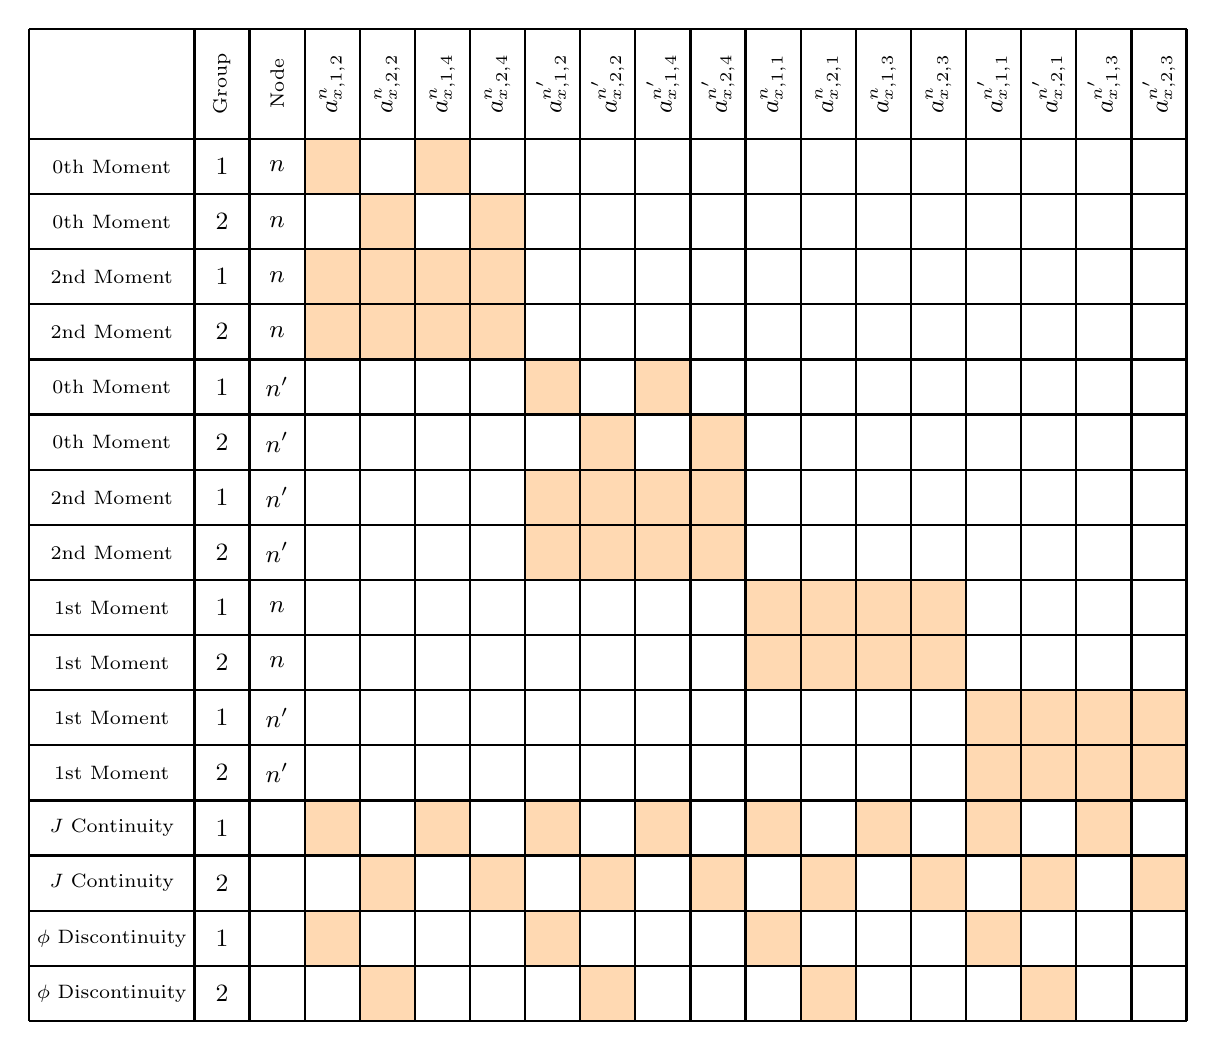
\begin{tikzpicture}[scale=0.7]


\fill[fill=orange!30] ( 2,15) -- ( 3,15) -- ( 3,16) -- ( 2,16) -- cycle;
\fill[fill=orange!30] ( 4,15) -- ( 5,15) -- ( 5,16) -- ( 4,16) -- cycle;

\fill[fill=orange!30] ( 3,14) -- ( 4,14) -- ( 4,15) -- ( 3,15) -- cycle;
\fill[fill=orange!30] ( 5,14) -- ( 6,14) -- ( 6,15) -- ( 5,15) -- cycle;

\fill[fill=orange!30] ( 2,12) -- ( 6,12) -- ( 6,14) -- ( 2,14) -- cycle;


\fill[fill=orange!30] ( 6,11) -- ( 7,11) -- ( 7,12) -- ( 6,12) -- cycle;
\fill[fill=orange!30] ( 8,11) -- ( 9,11) -- ( 9,12) -- ( 8,12) -- cycle;

\fill[fill=orange!30] ( 7,10) -- ( 8,10) -- ( 8,11) -- ( 7,11) -- cycle;
\fill[fill=orange!30] ( 9,10) -- (10,10) -- (10,11) -- ( 9,11) -- cycle;

\fill[fill=orange!30] ( 6, 8) -- (10, 8) -- (10,10) -- ( 6,10) -- cycle;

\fill[fill=orange!30] (10, 6) -- (14, 6) -- (14, 8) -- (10, 8) -- cycle;

\fill[fill=orange!30] (14, 4) -- (18, 4) -- (18, 6) -- (14, 6) -- cycle;

\fill[fill=orange!30] ( 2, 3) -- ( 3, 3) -- ( 3, 4) -- ( 2, 4) -- cycle;
\fill[fill=orange!30] ( 4, 3) -- ( 5, 3) -- ( 5, 4) -- ( 4, 4) -- cycle;
\fill[fill=orange!30] ( 6, 3) -- ( 7, 3) -- ( 7, 4) -- ( 6, 4) -- cycle;
\fill[fill=orange!30] ( 8, 3) -- ( 9, 3) -- ( 9, 4) -- ( 8, 4) -- cycle;
\fill[fill=orange!30] (10, 3) -- (11, 3) -- (11, 4) -- (10, 4) -- cycle;
\fill[fill=orange!30] (12, 3) -- (13, 3) -- (13, 4) -- (12, 4) -- cycle;
\fill[fill=orange!30] (14, 3) -- (15, 3) -- (15, 4) -- (14, 4) -- cycle;
\fill[fill=orange!30] (16, 3) -- (17, 3) -- (17, 4) -- (16, 4) -- cycle;

\fill[fill=orange!30] ( 3, 2) -- ( 4, 2) -- ( 4, 3) -- ( 3, 3) -- cycle;
\fill[fill=orange!30] ( 5, 2) -- ( 6, 2) -- ( 6, 3) -- ( 5, 3) -- cycle;
\fill[fill=orange!30] ( 7, 2) -- ( 8, 2) -- ( 8, 3) -- ( 7, 3) -- cycle;
\fill[fill=orange!30] ( 9, 2) -- (10, 2) -- (10, 3) -- ( 9, 3) -- cycle;
\fill[fill=orange!30] (11, 2) -- (12, 2) -- (12, 3) -- (11, 3) -- cycle;
\fill[fill=orange!30] (13, 2) -- (14, 2) -- (14, 3) -- (13, 3) -- cycle;
\fill[fill=orange!30] (15, 2) -- (16, 2) -- (16, 3) -- (15, 3) -- cycle;
\fill[fill=orange!30] (17, 2) -- (18, 2) -- (18, 3) -- (17, 3) -- cycle;


\fill[fill=orange!30] ( 2, 1) -- ( 3, 1) -- ( 3, 2) -- ( 2, 2) -- cycle;
\fill[fill=orange!30] ( 6, 1) -- ( 7, 1) -- ( 7, 2) -- ( 6, 2) -- cycle;
\fill[fill=orange!30] (10, 1) -- (11, 1) -- (11, 2) -- (10, 2) -- cycle;
\fill[fill=orange!30] (14, 1) -- (15, 1) -- (15, 2) -- (14, 2) -- cycle;

\fill[fill=orange!30] ( 3, 0) -- ( 4, 0) -- ( 4, 1) -- ( 3, 1) -- cycle;
\fill[fill=orange!30] ( 7, 0) -- ( 8, 0) -- ( 8, 1) -- ( 7, 1) -- cycle;
\fill[fill=orange!30] (11, 0) -- (12, 0) -- (12, 1) -- (11, 1) -- cycle;
\fill[fill=orange!30] (15, 0) -- (16, 0) -- (16, 1) -- (15, 1) -- cycle;


\foreach \i in {-3,0,1,...,18} {
  \foreach \j in {0,...,15,16,18} {
    \draw[thick] (-3,{\j}) -- (18,{\j});
    \draw[thick] ({\i},0) -- ({\i},18);
  }
}

\node at (-1.5,15.5) {\scriptsize 0th Moment};
\node at (-1.5,14.5) {\scriptsize 0th Moment};
\node at (-1.5,13.5) {\scriptsize 2nd Moment};
\node at (-1.5,12.5) {\scriptsize 2nd Moment};
\node at (-1.5,11.5) {\scriptsize 0th Moment};
\node at (-1.5,10.5) {\scriptsize 0th Moment};
\node at (-1.5, 9.5) {\scriptsize 2nd Moment};
\node at (-1.5, 8.5) {\scriptsize 2nd Moment};
\node at (-1.5, 7.5) {\scriptsize 1st Moment};
\node at (-1.5, 6.5) {\scriptsize 1st Moment};
\node at (-1.5, 5.5) {\scriptsize 1st Moment};
\node at (-1.5, 4.5) {\scriptsize 1st Moment};
\node at (-1.5, 3.5) {\scriptsize $J$ Continuity};
\node at (-1.5, 2.5) {\scriptsize $J$ Continuity};
\node at (-1.5, 1.5) {\scriptsize $\phi$ Discontinuity};
\node at (-1.5, 0.5) {\scriptsize $\phi$ Discontinuity};

\node[rotate=90] at (0.5,17) {\scriptsize Group};
\node[rotate=90] at (1.5,17) {\scriptsize Node};

\node at (0.5,15.5) {\small 1};
\node at (0.5,14.5) {\small 2};
\node at (0.5,13.5) {\small 1};
\node at (0.5,12.5) {\small 2};
\node at (0.5,11.5) {\small 1};
\node at (0.5,10.5) {\small 2};
\node at (0.5, 9.5) {\small 1};
\node at (0.5, 8.5) {\small 2};
\node at (0.5, 7.5) {\small 1};
\node at (0.5, 6.5) {\small 2};
\node at (0.5, 5.5) {\small 1};
\node at (0.5, 4.5) {\small 2};
\node at (0.5, 3.5) {\small 1};
\node at (0.5, 2.5) {\small 2};
\node at (0.5, 1.5) {\small 1};
\node at (0.5, 0.5) {\small 2};

\node at (1.5,15.5) {\small $n$};
\node at (1.5,14.5) {\small $n$};
\node at (1.5,13.5) {\small $n$};
\node at (1.5,12.5) {\small $n$};
\node at (1.5,11.5) {\small $n'$};
\node at (1.5,10.5) {\small $n'$};
\node at (1.5, 9.5) {\small $n'$};
\node at (1.5, 8.5) {\small $n'$};
\node at (1.5, 7.5) {\small $n$};
\node at (1.5, 6.5) {\small $n$};
\node at (1.5, 5.5) {\small $n'$};
\node at (1.5, 4.5) {\small $n'$};

\node[rotate=90] at ( 2.5,17) {\small $a_{x,1,2}^{n}$};
\node[rotate=90] at ( 3.5,17) {\small $a_{x,2,2}^{n}$};
\node[rotate=90] at ( 4.5,17) {\small $a_{x,1,4}^{n}$};
\node[rotate=90] at ( 5.5,17) {\small $a_{x,2,4}^{n}$};
\node[rotate=90] at ( 6.5,17) {\small $a_{x,1,2}^{n'}$};
\node[rotate=90] at ( 7.5,17) {\small $a_{x,2,2}^{n'}$};
\node[rotate=90] at ( 8.5,17) {\small $a_{x,1,4}^{n'}$};
\node[rotate=90] at ( 9.5,17) {\small $a_{x,2,4}^{n'}$};
\node[rotate=90] at (10.5,17) {\small $a_{x,1,1}^{n}$};
\node[rotate=90] at (11.5,17) {\small $a_{x,2,1}^{n}$};
\node[rotate=90] at (12.5,17) {\small $a_{x,1,3}^{n}$};
\node[rotate=90] at (13.5,17) {\small $a_{x,2,3}^{n}$};
\node[rotate=90] at (14.5,17) {\small $a_{x,1,1}^{n'}$};
\node[rotate=90] at (15.5,17) {\small $a_{x,2,1}^{n'}$};
\node[rotate=90] at (16.5,17) {\small $a_{x,1,3}^{n'}$};
\node[rotate=90] at (17.5,17) {\small $a_{x,2,3}^{n'}$};


\end{tikzpicture}
\end{center}

\caption{Matrix fill layout for a two-node problem with the nodal expansion method with a fourth-order expansion.}
\label{Fig:diffusion_NodalExpansion_2Node2Group_SparsityPattern}
\end{center}
\end{figure}

Typically we apply the nodal expansion method for a set of two adjacent nodes, corresponding to each interface between them. We also often solve the problem with two energy groups. In this case, there are three moment equations per node per group, and then the current continuity and flux discontinuity equations per group. This gives a total of 16 equations that need to be solved for a total of 16 coefficients: fourth coefficients per node per group.

These 16 equations and coefficients can be ordered such that the matrix has a convenient structure that is amenable for numerical linear algebra techniques. The ordering scheme and the matrix fill pattern is given in Fig.~\ref{Fig:diffusion_NodalExpansion_2Node2Group_SparsityPattern}. Here the shaded blocks represent that the coefficient is present in the given equation. Note again that node $n'$ is to the right (or above) node $n$ in our two-node problem.

This 16$\times$16 matrix can be solved using various numerical linear algebra techniques. Since two-group problems are quite common, many codes run a symbolic manipulator to obtain (very long) analytical expressions for the solution of each coefficient. These arithmetic expressions can then be optimized by the compiler to achieve superior computational speed.



\subsection{Coarse-Mesh Finite Difference Solution}

The solution scheme used by production methods couple nodal expansion and CMFD methods in a high-order, low-order coupling scheme. 

To begin, we note that the quantity of interest are the node-averaged scalar fluxes, which are used (along with the discontinuity factors) in conjunction with the transport calculations discussed in the previous chapter to reconstruct the detailed flux distribution within the core on the pin level. We note the nodal expansion method gives greater resolution within each node (assembly), but at a higher computational cost. The CMFD method applies the finite difference scheme on the node (assembly) resolution with an equivalence coefficient $\widehat{D}$ to enforce consistency between the currents, along with power iteration for the eigenvalue solve. The nodal expansion method is therefore the high-order scheme and CMFD is the low-order scheme.

The low-order CMFD scheme computes the node-averaged scalar fluxes $\overline{\phi}$ and the eigenvalue $k$. The results of these can also be used to compute the currents or transverse leakages $\overline{L}_x, \overline{L}_y, \overline{L}_z$ by taking their difference. 

These quantities are input into the high-order nodal expansion method for the two-node problem. The node-average fluxes and transverse leakages are source terms on the right-hand side of the nodal balance equation and the eigenvalue $k$ is embedded in the coefficient $A$ and within the aforementioned source. The solution of the two-node nodal expansion method are the coefficients, which can then be used to reconstruct the currents using Fick's law or Eq.~\eqref{Eq:diffusion_nodalExpansionMethod_4thOrder_Currents}. 

This current can then be used to compute an updated equivalence coefficient. For example if we assume discontinuity factors of unity, for an adjoining face in the $x$ direction we have
\begin{align}
  \widehat{D}_{i+1/2,j,g} = \frac{ -\overline{J}_{x,i+1/2,j,g}^{\text{NEM}} - \widetilde{D}_{i+1/2,j,g} ( \overline{\phi}_{i+1,j,g} - \overline{\phi}_{i,j,g} ) }{ \overline{\phi}_{i,j,g} + \overline{\phi}_{i+1,j,g} } .
\end{align}
Here the current $J$ is from the nodal-expansion method and $\widetilde{D}$ is the edge-averaged diffusion coefficient from the finite difference method. This equivalence coefficient is then used in the CMFD scheme to update the variable currents using, for example,
\begin{align}
  J_{x,i+1/2,j,g} = -\widetilde{D}_{i+1/2,j,g} \left( \overline{\phi}_{i+1,j,g} - \overline{\phi}_{i,j,g} \right) - \widehat{D}_{i+1/2,j,g} \left( \overline{\phi}_{i+1,j,g} + \overline{\phi}_{i,j,g} \right) .
\end{align}
Applying this to the 3-D balance equation for node $(i,j,k)$, we have
\begin{align}
  &\frac{1}{\Delta x_{i}} \bigg[ -\widetilde{D}_{i+1/2,j,k,g} \left( \overline{\phi}_{i+1,j,k,g} - \overline{\phi}_{i,j,k,g} \right) - \widehat{D}_{i+1/2,j,k,g} \left( \overline{\phi}_{i+1,j,k,g} + \overline{\phi}_{i,j,k,g} \right) \nonumber \\*
 &+ \widetilde{D}_{i-1/2,j,g} \left( \overline{\phi}_{i,j,k,g} - \overline{\phi}_{i-1,j,k,g} \right) + \widehat{D}_{i-1/2,j,k,g} \left( \overline{\phi}_{i,j,k,g} + \overline{\phi}_{i-1,j,k,g} \right) \bigg] \nonumber \\*
  &\frac{1}{\Delta y_{j}} \bigg[ -\widetilde{D}_{i,j+1/2,k,g} \left( \overline{\phi}_{i,j+1,k,g} - \overline{\phi}_{i,j,k,g} \right) - \widehat{D}_{i,j+1/2,k,g} \left( \overline{\phi}_{i,j+1,k,g} + \overline{\phi}_{i,j,g} \right) \nonumber \\*
 &+ \widetilde{D}_{i,j-1/2,k,g} \left( \overline{\phi}_{i,j,k,g} - \overline{\phi}_{i,j-1,k,g} \right) + \widehat{D}_{i,j-1/2,k,g} \left( \overline{\phi}_{i,j,k,g} + \overline{\phi}_{i,j-1,k,g} \right) \bigg] \nonumber \\* 
  &\frac{1}{\Delta z_{k}} \bigg[ -\widetilde{D}_{i,j,k+1/2,g} \left( \overline{\phi}_{i,j,k+1,g} - \overline{\phi}_{i,j,k,g} \right) - \widehat{D}_{i,j,k+1/2,g} \left( \overline{\phi}_{i,j,k+1,g} + \overline{\phi}_{i,j,k,g} \right) \nonumber \\*
 &+ \widetilde{D}_{i,j,k-1/2,g} \left( \overline{\phi}_{i,j,k,g} - \overline{\phi}_{i,j,k-1,g} \right) + \widehat{D}_{i,j,k-1/2,g} \left( \overline{\phi}_{i,j,k,g} + \overline{\phi}_{i,j,k-1,g} \right) \bigg] \nonumber \\* 
 &+ \Sigma_{R,i,j,k,g} \overline{\phi}_{i,j,k,g} = q_{i,j,k,g} .
\end{align}
While this equation appears unwieldy, we can factor it out into an expression that couples the neighboring nodes. We can then flatten the spatial indices as with the 2-D case, here $m = i + (j-1) N_x + (k-1) N_x N_y$, and then form a large matrix that can be solved using iterative schemes for each energy group. The same treatment for upscattering and power iteration of the fission source applies here. We then use the solution to these CMFD equations, the volume-averaged scalar fluxes, the currents, and the eigenvalue $k$, to compute the inputs for the nodal expansion method for each interface.

The algorithm proceeds as follows. First, we assume a zero equivalence coefficient $\widehat{D} = 0$ everywhere. We then obtain a solution to the CMFD equations to find the node-average fluxes, transverse leakages, and eigenvalue. We then feed these as input into a series of two-node nodal expansion calculations, one for each nodal interface. The result of each of these nodal calculations are the coefficients that are used to calculate an update current and new $\widehat{D}$. We then return to performing CMFD calculations with the updated $\widehat{D}$ to obtain new node-average scalar fluxes, etc. that are then used as input again into a series of two-node nodal expansion calculations. We repeat this process until the volume-averaged scalar fluxes, face-average fluxes, face-avarged currents, and eigenvalue $k$ converge.





\section{Pin-Power Reconstruction}

The nodal expansion methods provide node-averaged fluxes and interface currents for a diffusion problem with homogenized assemblies across the full core. This problem, however, only gives the gross flux shapes across the reactor and is mostly insufficient for making design decisions. For example, to ensure that fuel temperatures or heat fluxes are below safety limits (peak centerline temperature and critical heat flux), we need detailed pin-resolved powers as input into subchannel thermal hydraulics calculations.

The general idea is to merge together information from the full-core nodal diffusion calculations and assembly-level transport calculations. There are several approaches that have been developed over the years to do this and here we explain one such approach that is in a similar spirit to the nodal expansion method.

\subsection{2-D Node Flux Distribution}

The nodal expansion calculation applied transverse integration techniques leading to flux shapes along $x$, $y$, and $z$ independently. A natural choice for finding the 3-D power distribution is to assume the flux shape can be expressed as the product of these three functions. This would work if the flux solution is separable along each direction. Unfortunately, empirical evidence shows that such an approximation on the flux in the $x$ and $y$ directions is not suitable, whereas the axial dependence of the flux can be separated:
\begin{align}
  \phi_g(x,y,x) = \phi_g(x,y) \phi_g(z) .
\end{align}
Of course, we are now left with finding $\phi(x,y)$.

One such approach that is used for conventional reactors is to assume a functional form for the fast and thermal fluxes. For the fast flux, we assume a biquartic form:
\begin{align}
  \phi_1(x,y) = \sum_{m,n=0}^4 a_{m,n} x^m y^n .
\end{align}
The difference between a simple product of 1-D functions is that the cross terms have free-parameter coefficients. For the thermal flux, it has been empirically found that the following basis function:
\begin{align}
  \phi_2(x,y) = c_{0,0} \phi_1(x,y) + \sum_{\substack{m,n = 0\\ m = n \ne 0}} c_{m,n} F_m(x) F_n(y) ,
\end{align}
where
\begin{subequations}
\begin{align}
  F_0(u) &= 1, \\
  F_1(u) &= \sinh(  \kappa u ), \\
  F_2(u) &= \cosh(  \kappa u ), \\
  F_3(u) &= \sinh( 2\kappa u ), \\
  F_4(u) &= \cosh( 2\kappa u ),
\end{align}
where $u = x$ or $y$ and
\begin{align}
  \kappa^2 = \frac{ h^2 \Sigma_{a2} }{ D_2 } ,
\end{align}
\end{subequations}
with $h$ being the width of the node.

Before proceeding we pause and note that we assume the shape thermal flux is well described by the sum of the fast flux plus a series of hyperbolic trigonometric functions, or equivalently, exponentials. This fourth-order polynomial expansion for the fast flux is empirical, motivated by the fact that it works well enough in conventional reactors, and should not be expected to be adequate in general. The choice of basis of hyperbolic trigonometric functions (or equivalently exponentials) is also a bit empirical, although there is some mathematical justification in that it is a solution to the 2-D diffusion problem. A second important point is that the method is purely restricted to two energy groups, which again may be a major limitation depending on the needs of the overall analysis.

We now note that each expression for the fast and thermal fluxes involves 25 unknown coefficients. The nodal diffusion calculation provides 9 constraints: the volume-averaged scalar flux, the edge-averaged flux on each face, and the edge-averaged current on each face. We now require an additional 16 constraints to have a unique solution.



\subsection{Corner Fluxes}

We can obtain four additional constraints if we somehow know the fluxes at the node corners. There are a couple ways one could do this, but perhaps the simplest approach is to assume that the flux $\phi(x,y)$ is separable only at the corners (as opposed to the entire domain), 
\begin{align}
  \phi(x_{i+1/2},y_{j+1/2}) \approx \frac{ \phi_x(x_{i+1/2}) \phi_y(y_{j+1/2}) }{ \overline{\phi}_{i,j} } .
\end{align}
Given this, we can directly use the transverse integrated fluxes from the nodal diffusion calculations.

If the adjoining nodes are identical homogenized assemblies, then there is no ambiguity about the value of the flux at the corner point. Typically though, we have different assemblies and the fluxes from the nodal diffusion calculations in these adjoining nodes will not be identical at the corners. One option is to simply average the nodal diffusion fluxes across the four adjoining assemblies, but this is not physically motivated. 

The reconstructed heterogeneous fluxes, however, must be continuous everywhere throughout the reactor, therefore we could average the predicted values of these heterogeneous fluxes. Within each heterogeneous assembly, we assume we have a \emph{flux form function} $\Phi$ that is obtained from an assembly-level transport calculation. Taking the average across the assemblies we have
\begin{align}
  \phi(x_{i+1/2},y_{j+1/2}) = \frac{1}{4} \frac{ \phi_{i,j} \Phi_{i,j} + \phi_{i,j} \Phi_{i,j} + \phi_{i,j} \Phi_{i,j} + \phi_{i,j} \Phi_{i,j} }{ \Phi_{i,j} } ,
\end{align}
where all quantities on the right-hand side are evaluated at the corner point. 

A better approach is to calculate \emph{corner discontinuity factors}. These new discontinuity factors can be obtained in a similar manner as the assembly discontinuity factors at the edges: by taking the ratio of the corner flux to the volume-averaged flux in the assembly. We then perform a calculation about the node corner applying the corner discontinuity factor there.

In either case, once we have the fluxes at the corners, we now can impose the four additional constraints.




\subsection{Reconstruction Method}

With the additional four corner fluxes, we now have a total of 13 constraints, but still 25 unknowns, per energy group. We can now impose an additional approximation onto the flux expansion. Observe 13 constraints gives enough information to determine the monomial coefficients in $x$ and $y$ up to order 4, for a total of 9 coefficients (noting that the constant is a single coefficient), plus the coefficients in $xy$, $x^2 y$, $x y^2$, and $x^2 y^2$, bringing us to 13. 

One option is to neglect all of the other terms, setting the coefficients on all cross terms where $m, n > 2$ to zero. In practice, this empirical approach well describes the 2-D flux distribution within a node---at least well enough for conventional reactors. Having a well posed problem, we can now proceed with solving for the coefficients to describe the flux shape within the node.

To get the power from the flux, we require one additional quantity from the assembly transport calculation, a \emph{power form function} $\Pi$. This is essentially the same as the flux form function, but scaled by the local energy release per fission times the fission cross section and summed over the energy groups. The local power is then
\begin{align}
  P(x,y) =  \Pi(x,y) \left[ \Sigma_{f1} \phi_1(x,y) +  \Sigma_{f1}  \phi_2(x,y) \right] .
\end{align}




%%%%%%%%%%%%%%%%%%%%%%%%%%%%%%%%%%%%%%%%%%%%%%%%%%%%%%%%%%%%%%%%%%%%%%%%%%%%%%%%
\section{Depletion Calculations}

Over time the inventory of fissionable nuclides in the reactor depletes. When neutrons cause fission, the fuel isotope is split into two fragments. These fragments are usually radioactive and undergo decay, which generates further heat. While this thermal energy from repeated radioactive decay needs to be removed continuously for years to prevent the fuel from overheating, it is not sufficient to drive an energy conversion cycle. Therefore, these radioactive fragments are a waste byproduct of fission that must be managed. From the reactor's perspective, each fission means one less fissionable nuclide and there is a reduction in the total amount of excess reactivity in the reactor. 

The buildup of fission product poisons and the associated oscillations is on the timescale of hours and days. On the longer timescale of weeks or months, the depletion of the fuel via fission or burnable absorbers via capture must be considered. On one hand. the depletion of fuel decreases the reactivity because there is less fissionable material. On the other, the depletion of the burnable absorbers increases the reactivity because once they capture neutrons they lose their ability to capture further neutrons. Additionally, the fuel of power reactors consists primarily $^{238}$U, which is responsible for much of the absorption of neutrons. This neutron capture reaction produces $^{239}$U, which rapidly decays to $^{239}$Np, and after about 2.4 days, decays into $^{239}$Pu, which is itself fissile. Furthermore, this inventory of $^{239}$Pu captures neutrons to make $^{240}$Pu and then can capture another to make $^{241}$Pu, and so on. We refer to this as the conversion of fertile isotopes and is a long-term increase in reactivity (so long as we do not run out of fertile material.)

On balance, a typical thermal reactor has enough fuel and excess reactivity to sustain operations for about 18-24 months before new fuel needs to be cycled into the reactor. In other words the depletion of fuel dominates the production of fissile isotopes from conversion. At the end of a typical reactor cycle, about a third of the power comes from various Pu isotopes.

\begin{figure}[tb!]
\begin{center}
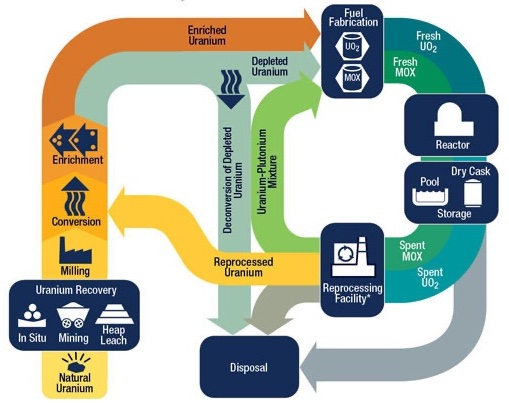
\includegraphics[width=0.8\textwidth]{./Figures/NRCFuelCycle.jpg}
\caption{Illustration of the nuclear fuel cycle (US Nuclear Regulatory Commission)}
\label{Fig:kinetics_nuclearFuelCycle}
\end{center}
\end{figure}

Before going into the analysis of the reactor, it is helpful to zoom out to the big picture of how the entire nuclear fuel cycle functions. This is depicted in Fig.~\ref{Fig:kinetics_nuclearFuelCycle}.

Before going into details, there are two primary types of fuel cycles in use. The US uses a once-through fuel cycle where fuel is put into a reactor, burned, and then disposed of as waste. France and Japan, on the other hand, perform fuel recycling, extracting the plutonium and blending it with uranium fuel to make mixed-oxide or MOX fuel assemblies that are then put back into reactors for additional burnup. 

The advantages of recycling is that it has a greater resource utilization and reduces the quantity of spent nuclear fuel that must be managed. The disadvantage is this comes at an increased cost, as mining uranium is inexpensive. Second, there is an increased risk of diversion of weapons usable materials. While reactor grade plutonium contains too much $^{240}$Pu to be an ideal nuclear explosive and is not the most attractive route for a nation state to pursue, it is nonetheless possible to use it for that purpose. This increased risk must be offset by increased costs to minimize the possibilities of such fuel diversions.

The once-through nuclear fuel cycle consists of the following major steps:
\begin{enumerate}
  \item Mining -- uranium is obtained by extracting it from ores underground resources. Like all mining, this is a polluting industry and is arguably the most environmentally damaging part of the nuclear fuel cycle. The argument in favor is because of the energy density of nuclear fuels, we require less mining than other energy sources.
  \item Milling -- the raw uranium ore must be extracted and comes in the composition of U$_3$O$_8$, which is sometimes called yellowcake. 
  \item Conversion -- in the US, fuel must be enriched and U$_3$O$_8$ is not a chemical form that permits this. We convert it into UF$_6$, which readily enters a gaseous phase.
  \item Enrichment -- the gaseous UF$_6$ is put into fast moving centrifuges. Because of the small mass differential between $^{235}$U and $^{238}$ the centrifugal forces preferentially push one isotope out more than other. The stock is moved through a series of such centrifuges until a desired enrichment (usually a few percent) is reached.
  \item Fuel Fabrication -- the enriched UF$_6$ is converted into ceramic UO$_2$ and sintered into pellets and sealed into fuel cladding tubes. These fuel rods are then put into bundles or assembles that are delivered to a power plant.
  \item Reactor -- the fuel is put into the reactor and is used to cause fission, producing thermal and then electrical energy. A typical fuel assembly resides in the reactor between 3-6 years.
  \item Onsite Storage -- once the fuel is sufficiently depleted it is moved out of the reactor for storage. Because of the large inventory of fission products, the fuel continues to generate a large amount of heat because of radioactive decay that must be removed. This is done by placing them into a spent fuel pool where the fuel assembly resides for several years. Once the radioactive inventory has decreased enough, the fuel is moved out of the pool and placed in dry casks that are cooled with air.
  \item Long-term Repository -- while not yet in operation, the plan in the US is to move the fuel in the spent fuel casks into a long-term or permanent repository for final disposition.
\end{enumerate}
 
In a fuel-recycle scenario, sometime after the fuel is removed from the reactor, it is sent to a reprocessing facility where it is chemically dissolved and separated. The plutonium is extracted and then mixed with uranium to create fuel with enough reactivity to go back into a reactor. The recycling process produces waste that must similarly be disposed of, but the volume and radiotoxicity is much less. 

More advanced fuel cycles are currently being investigated that make use of fast reactors that are capable of burning up the fissionable (but not fissile) actinides with long half lives that account for much of the radiotoxicity on the 1,000 to 100,000 year timeframe. While the technology is theoretically in place, it has yet to be demonstrated in an economically competitive manner.

\subsection{Burnup and Conversion Ratio}

Zooming back into the reactor eventually, the fuel becomes too depleted to effectively sustain a chain reaction and must be removed from the reactor. This can be mitigated by reshuffling the fuel and mixing it with fresh fuel assemblies, but there are still limits. The limiting factor is not the availability of fuel per se, but rather the fuel experiences steady damage from the energetic fission fragments. Additionally, the buildup of these fragments changes the chemistry, leading to corrosive chemical interactions with the cladding. Also, some of the fission products are gases and these fill the sealed fuel-cladding tube and lead to an increase in internal pressure. As the fuel continues to burn up, its structural integrity diminishes and the probability of fuel failure increases with time. Therefore, fuel inventory concerns aside, it is necessary to remove the fuel from the reactor after a few years lest the fuel rods begin to fail and leak fission products into the coolant.

We quantify the fuel exposure to neutrons with a quantity called \emph{burnup}, which is defined as
\begin{align}
  BU = \frac{\text{energy released from fission}}{\text{mass of the fissionable material}} .
\end{align}
Typically we express the energy in units of GWd (GigaWatt days), based on the thermal (not electrical) power of the reactor, and the units of mass as MTU, metric tons of uranium (excluding the mass of oxygen in the conventional UO$_2$ fuel). If different fissionable materials are used, then the mass needs to adjusted accordingly and sometimes the denominator is quoted as mass of heavy metal. Further, the mass of fissionable material typically includes all isotopes, not just, for example, the fissile $^{235}$U.

Typical end-of-life burnups for conventional UO$_2$ fuel is between 30 to 40 GWd/MTU. In recent years, there has been considerable effort to developing fuel capable of handling higher burnup, up to around 60 GWd/MTU, which means they can stay in the reactor longer and more energy can be extracted per unit mass. Advanced reactors such as gas-cooled variants use spherical TRISO fuel kernels that are capable of even higher fuel burnups.

As mentioned, some of the fertile $^{238}$U in a reactor is converted into fissile plutonium isotopes. In a conventional reactor, the depletion of $^{235}$U cannot keep up with the creation of plutonium. However, it is possible to create more fuel than is burned in a \emph{breeder reactor}. For thermal reactors, we use a thorium-based cycle where the fertile $^{232}$Th captures neutrons and produces (after a couple $\beta^-$ decays) fissile $^{233}$U, which is the actual fuel. In fast reactors, we typically convert $^{238}$U into Pu isotopes in an external blanket that can then be extracted, chemically separated, and used to make more fuel for other reactors. In the early days of nuclear power, the known resources of uranium was thought to be much more limited than it actually is. Today, there is a large supply of economically mineable uranium resources such that the resource question is far less of an short or medium term concern. That said, there is still interest in thorium cycles or fast reactors, but these are driven by other factors rather than long-term uranium resources.

Regardless of whether the intent is to breed new fuel, some will be produced and this quantity is called the \emph{conversion ratio}. This is
\begin{align}
  CR = \frac{\text{production rate of fissile atoms}}{\text{consumption rate of fissile atoms}} .
\end{align}
In a conventional reactor, the conversion ratio is less than one, i.e., the fuel is burned faster than it is produced. For a typical thermal power reactor, this conversion ratio is on the order of 0.5 to 0.6. In a breeder reactor, the conversion ratio is greater than one and is then usually called the \emph{breeding ratio}.




\subsection{Depletion Equations} \label{Sec:kinetics_fuelDepletionEquations}

Analyzing the depletion of the reactor is actually a very complicated process. Modern methods typically consider every reaction pathway and fission product individually, considering their radioactive decay. This is done by solving the rate equations including depletion and production, which is a series of first-order ordinary differential equations in each spatial region that depends on the local scalar flux $\phi(\pos,t)$. 

The general form of the rate equation in a reactor for isotope $i$ with concentration $N_i$ is
\begin{align}
  \frac{dN_i}{dt} &= 
  \underbrace{\sum_j \lambda_{ji} N_j(t) }_{\parbox{2.25cm}{\scriptsize rate isotope $i$ is produced from radioactive decay of all isotopes $j$}}
  + \underbrace{\sum_g \sum_j \gamma_{ji} \sigma_{f,g,j} \phi_g(t) N_j(t)}_{\parbox{3.5cm}{\scriptsize rate isotope $i$ is produced from fission from all fissionable isotopes $j$}}
  + \underbrace{\sum_g \sum_j \sigma_{g,ji} \phi_g(t) N_j(t)}_{\parbox{2.75cm}{\scriptsize rate isotope $i$ is produced from all non-fission nuclear reactions with isotopes $j$}} \nonumber \\*
  &- \underbrace{\sum_g \sum_x \sigma_{x,g,i} \phi_g(t) N_i(t)}_{\parbox{3cm}{\scriptsize rate isotope $i$ is removed because of all nuclear reactions $x$}}
  - \underbrace{\lambda_i N_i(t) }_{\parbox{1.75cm}{\scriptsize rate isotope $i$ is removed by radioactive decay}}.
\end{align}
Here
\begin{align}
  \lambda_{ji} &= \text{decay constant for isotope $j$ decaying to isotope $i$},  \nonumber \\
  \gamma_{ji}  &= \text{fission product yield for isotope $i$ from fissionable nucleus $j$}, \nonumber \\
  \sigma_{g,ji}  &= \text{reaction cross section for conversion from isotope $j$ into $i$ for energy group $g$}, \nonumber \\
  \sigma_{x,g,i} &= \text{cross section for reaction $x$ of isotope $i$ for energy group $g$}, \nonumber \\
  \lambda_i    &= \text{decay constant for isotope $i$ (for all decays)}. \nonumber 
\end{align}
An equation is written down for each isotope $i$. These equations can then be formed into a linear system as
\begin{align}
  \frac{d\mathbf{N}}{dt} = \mathbf{A}(t) \mathbf{N}(t) ,
\end{align}
where the coefficient matrix $\mathbf{A}$ depends on both the nuclear data and the local scalar flux $\phi(t)$, which carries the time dependence of the matrix.






\subsection{Burnup Flux Spectrum}

The depletion equations require knowledge of the reactor scalar flux within each region. Over the course of performing reactor analyses, we obtained several fluxes for various energy and spatial resolutions and we need to find an appropriate one to use. A typical process involves obtaining the leakage-corrected spectrum at the reflected assembly level, i.e., not using the full core nodal diffusion calculations, by using the $B_1$ spectra with the finely resolved, in both space and energy, transport fluxes that are scaled to the reactor power. The general process goes as follows:
\begin{enumerate}
  \item use the $B_1$ flux spectrum to rebalance the coarse-group assembly transport calculated fluxes;
  \item expand the coarse group flux spectra with the pin-level fine-group transport spectra;
  \item scale the fluxes to the reactor power.
\end{enumerate}

The first step is to perform the rebalance with the $B_1$ spectra for the homogenized assembly. As with the process to determine the few-group constants for the nodal diffusion calculations, the $B_1$ calculation adjusts the infinitely reflected assembly transport spectrum to account for the fact that in an actual reactor there must be a balance from either outflow (for a supercritical infinitely reflected assembly) or inflow (for a subcritical one) of neutrons from neighboring assemblies.

We define $\phi_{B,g}$ as the $B_1$ infinite medium spectrum for fine energy group $g$ and $\phi_{I,c}$ to be the flux spectrum within spatial region $I$ and coarse energy group $c$ from the assembly transport calculation. The leakage-corrected coarse-group spectrum is
\begin{subequations}
\begin{align}
  \phi_{L,I,c} = \frac{ \phi_{B,c} }{ \overline{\phi}_c } \phi_{I,c}
\end{align}
Here
\begin{align}
  \phi_{B,c} &= \sum_{g \in c} \phi_{B,g} \\
  \overline{\phi}_c &= \dfrac{ \displaystyle\sum_I \phi_{I,c} V_I }{ \displaystyle\sum_I V_I } .
\end{align}
\end{subequations}

We then expand the coarse groups into the fine groups. We let $\phi_{i,g}$ be the fluxes in fine-spatial region $i$ and fine-energy group $g$ from the pin-level collision probability/response matrix transport calculations. We then obtain the fine leakage-corrected flux spectra as
\begin{align}
  \phi_{L,i,g} = \dfrac{ \phi_{L,I,c} V_I }{ \displaystyle\sum_{i' \in I} V_{i'} \sum_{g' \in c} \phi_{i',g'} } \phi_{i,g} .
\end{align}

The final step in the process is to scale these fluxes by the power level to obtain $\phi_{P,i,g}$, the scaled fine fluxes. This is done by using
\begin{subequations}
\begin{align}
  \phi_{P,i,g} = \left[ \dfrac{ P M_0 }{ \displaystyle\sum_{i \in F} V_i \overline{\phi}_{L,i} \sum_j N_{j,i} \epsilon_j \overline{\sigma}_{f,j,i}  } \right] \phi_{L,i,g} ,
\end{align}
where
\begin{align}
  P &= \text{power density in units of watts per gram of fissionable material},  \nonumber \\
  M_0  &= \text{initial (pre-burnup) mass of fissionable material in units of grams}, \nonumber \\
  V_i  &= \text{volume of region $i$ within fuel $F$ in cm$^3$}, \nonumber \\
  \overline{\phi}_{L,i} &= \text{energy-integrated, leakage-corrected flux spectrum in region $i$ in cm$^{-2}$ s$^{-1}$}, \nonumber \\
  j    &= \text{index for fissionable isotope}, \nonumber \\
  N_{j,i} &= \text{atomic density of fissionable isotope $j$ within region $i$ in $10^{24}$ cm$^{-3}$}, \nonumber \\
  \epsilon_j &= \text{energy release per fission in Watt-seconds per fission}, \nonumber \\
  \overline{\sigma}_{f,j,i}    &= \text{spectrum-averaged fission cross section for isotope $j$ in $10^{-24}$ cm$^2$}. \nonumber 
\end{align}
The initial fissionable mass is calculated by
\begin{align}
  M_0 = \sum_{i \in F} V_i \sum_j N_{0,j,i} m_j ,
\end{align}
where $N_{0,j,i}$ is the initial (pre-burnup) atomic density in units of atoms per cm$^{3}$ times the mass $m_j$ in grams per atom. The energy-integrated leakage spectrum is calculated using
\begin{align}
  \overline{\phi}_{L,i} = \sum_g \phi_{L,i,g} .
\end{align}
The spectrum-averaged fission cross section is computed from
\begin{align}
  \overline{\sigma}_{f,j,i} &= \dfrac{ \displaystyle\sum_g \sigma_{f,j,i,g} \phi_{L,i,g} }{ \overline{\phi}_{L,i} } .
\end{align}
\end{subequations}

Once we have $\phi_P$ for each region and energy group, we then numerically solve the depletion equations. From here on in this section we drop the subscript $P$ as it is the implied flux spectrum in all depletion calculations.





\subsection{Predictor-Corrector Method}

If we assume that the scalar flux is constant over some time interval, i.e., a time step in a calculation $t_i \le t < t_{i+1}$, then this system has a solution as the matrix exponential,
\begin{align}
  \mathbf{N}(t) = \exp\left[ (t-t_i) \mathbf{A} \right] \mathbf{N}(t_i) , \quad t_i \le t < t_{i+1} ,
\end{align}
where $\mathbf{N}(t_i)$ is a known initial condition at $t = t_i$, the beginning of the interval. 

In practice this forward Euler scheme is not what is actually used. The complication that arises is similar to that of the fission product poisons in that the changes in local isotopics leads to a change in the local flux. This means that the depletion equations are non-linear and need to be solved numerically on a time grid that is fine enough to capture the temporal changes of the isotopic concentrations. 

The typical numerical scheme used is called the \emph{predictor-corrector method}. The idea is to break the reactor fueling cycle into a series of time steps that are sufficiently small to capture any changes in the reactor conditions. Typically, this means we need a relatively short time step or two to account for the buildup to the equilibrium states of the fission product poisons $^{135}$Xe and $^{149}$Sm every time the reactor changes its power level. Then, we need to take time steps of on the order of a few weeks to capture slower, long term fuel depletion and fertile conversion effects.

Suppose the isotopic compositions are known at the beginning of time step $t_i$ and given in a vector $\mathbf{N}(t_i)$ . We can then solve the neutron transport or diffusion equations using these componsitions with some numerical scheme to get the consistent scalar fluxes. We call these $\phi_1(t_i)$.

We then plug the scalar flux $\phi_1(t_i)$ into the system of rate equations and solve them at each position in the reactor to arrive at a \emph{prediction} of the new isotopic composition vector $\hat{\mathbf{N}}(t_i)$. We could use this prediction as the new isotopic compositions $\mathbf{N}(t_{i+1})$, but it turns out doing this, wile simple, would require taking very large time steps.

Instead, we use this new vector as input into the neutron transport and diffusion equation and solve for an updated scalar flux using the new compositions that we call $\phi_2(\pos,t_i)$. We then go back and compute a \emph{corrected} isotopic composition by using the average of the scalar fluxes,
\begin{align}
  \phi(t_i) = \frac{ \phi_1(t_i) + \phi_2(t_i) }{ 2 } ,
\end{align}
as the scalar flux to compute $\mathbf{N}(t_{i+1})$. We then use this as the initial condition of for the next time step. Because the core composition has changed, we then need to perform a criticality search after each time step based on changing control rod heights or soluble boron concentrations.

Note again that these equations must be solved for all locations in the reactor, so it can become a rather computationally taxing task for a large reactor with numerous fuel pins. Using the predictor-corrector method significantly improves the accuracy of the depletion solve over forward Euler and allows for taking much larger time steps than would be possible otherwise. More sophisticated methods exist, and finding better depletion solver techniques that balance accuracy versus computational costs remains an open area of study.

One thing worth mentioning is that the coefficients in the matrix $\mathbf{A}$ span several orders of magnitude. This implies we have phenomena that occur on timescales ranging from milliseconds to millions of years. It turns out that evaluating the matrix exponential is actually difficult in this case because of numerical precision issues. While this problem has not completely gone away, the last few decades have seen advances in numerical solution techniques capable of handing what we term stiff systems of differential equations, and the issue is far less acute than it used to be.


